%!TEX root = /Users/jakubkonka/Thesis/Thesis.tex
\chapter{Direct Analysis of Network Selection Mechanism} % (fold)
\label{cha:direct}

\minitoc
\vspace{10mm}

This chapter formally defines the network selection mechanism in the Digital Marketplace (DMP), and casts it into the framework of game theory. The mechanism is then direcly analysed in three special cases: 1) when only reputation ratings of the network operators decide on the winning network operator, 2) when only the monetary bids of the network operators matter in the selection of the winner, and finally, 3) when all network operators are characterised by the same reputation rating. In essence, those special cases correspond to the extremes of the studied bidding problem, and in all those cases, the equilibrium bidding strategies are derived.

The chapter then concludes with the analysis of the mechanism in a restricted case with only two network operators, for which the equilibrium bidding strategies are derived. They are shown, however, to be suboptimal as they allow the network operators to submit a negative monetary bid.

\section{Problem Definition and Assumptions} % (fold)
\label{sec:problem_definition_and_assumptions_direct}
The formal description of the network selection mechanism employed in the DMP is as follows. The model is a modified version of procurement first-price sealed-bid auction (henceforth, we shall refer to procurement first-price sealed-bid auction as FPA). Thus, formally, it represents a Bayesian game of incomplete information\footnote{See Appendix~\ref{cha:notation} for the definition of a Bayesian game of incomplete information, and any other game theoretical and mathematical concepts used in this chapter.}, $\Gamma^B$. There are $n$ network operators who bid for the right to sell their product to the subscriber such that $n = |N|$ where $N$ denotes the set of all network operators.

Let $\beta : \mathbb{R}_+\times [0,1] \to \mathbb{R}_+$, defined by
\begin{equation}
	\label{eq:def_beta_direct}
	\beta(b_i, r_i) = w_{price}\cdot b_i + w_{penalty}\cdot r_i \quad\text{for all } i\in N,
\end{equation}
denote the compound bid. Each network operator $i$ is characterized by the utility function $u_i$ such that
\begin{equation}
	\label{eq:sellers_utility_direct}
	u_i(b,c,r) = \left\{
	\begin{array}{l l}
		b_i-c_i & \;\text{if } \beta(b_i, r_i) < \displaystyle\min_{j\neq i}\beta(b_j,r_j),\\
		0 & \;\text{if } \beta(b_i, r_i) > \displaystyle\min_{j\neq i}\beta(b_j,r_j),
	\end{array}\right.
\end{equation}
where $b = (b_i,b_{-i})$ represents the monetary bid (or offered price) vector, $c = (c_i, c_{-i})$ the type vector, and $r = (r_i, r_{-i})$ the reputation rating vector. The type of each network operator is assumed to represent the cost of (or the minimum price for) transporting the service request under consideration. The winner of the auction is determined as the network operator whose compound bid is the lowest one; i.e.,~network operator $i$ is the winner if
\begin{equation*}
	\beta(b_i, r_i) < \displaystyle\min_{j\neq i}\beta(b_j,r_j).
\end{equation*}
In the event that there is a tie
\begin{equation*}
	\beta(b_i, r_i) = \displaystyle\min_{j\neq i}\beta(b_j,r_j),
\end{equation*}
the winner is randomly selected with equal probability.

It is, moreover, assumed that the price and reputation weights $(w_{price}, w_{penalty})$ are announced by the subscriber to all network operators before the auction. Thus, there is no uncertainty in knowing how much the subscriber values the offered price of the service over the reputation of the network operator (or vice versa). Furthermore,
\begin{equation*}
	w_{price} + w_{penalty} = 1,\quad 0\le w_{price},w_{penalty} \le 1.
\end{equation*}
In order to simplify the notation, it is assumed throughout the rest of this thesis that $w=w_{price}$. This simplifies the definition of the compound bid in Equation~\eqref{eq:def_beta_direct} to
\begin{equation*}
  \beta(b_i, r_i) = wb_i + (1-w)r_i\quad\text{for all } i\in N.
\end{equation*}
Note, however, that this assumption could potentially lead to a situation where network operators manipulate the knowledge of $w$ to increase their profits by overcharging the subscriber. Therefore, in order to circumvent such an eventuality, the subscriber would only consider offers such that
\begin{equation}
	\label{eq:subscribers_valuation_direct}
	v\geq wb_i + (1-w)r_i \quad\text{for all } i\in N
\end{equation}
where $v\in (0,1]$ is the subscriber's valuation, and it is private knowledge~\cite{DMLeBodic00}. The subscriber's valuation is effectively equivalent to a secret (or hidden) reserve price~\cite{Vincent1995575,LiPerrigne1999,BajariHortacsu2003}. This creates an additional uncertainty about the auction that each network operator needs to incorporate into their equilibrium bidding strategies. To elaborate further, by setting a secret reserve valuation, the subscriber creates a phantom bidder characterized by a reputation rating $r_0$ and submitting a bid $b_0$ such that $v=\beta(b_0,r_0)$, and therefore, risks not obtaining a service offer from any network operator if $v < \beta(b_i,r_i)$ for all $i\in N$. Therefore, the solution presented in this and the following chapters would have to be modified by including the phantom bidder in the derivation of the equilibrium bidding strategies. However, in order to keep the analysis tractable, we do not incorporate this assumption in this research.
	
Following the standard assumptions from the auction literature~\cite{Krishna10}, the set of network operators, $N$, is finite and the network operators are risk neutral; that is, they seek to maximize their expected profits. Furthermore, the subscriber is risk neutral and does not have any budget constraints; that is, the subscriber is prepared to accept any offer from the network operators. In reality, it is unlikely for the network operators and the buyer to be risk neutral, and the buyer to not have any budget constraints. However, in order for the problem to be tractable, we enforce those assumptions in this research. The implications of relaxing those assumptions on the analysis of an auction are explored in Krishna~\cite{Krishna10}.

The costs $c_i$ for each network operator $i$ are private knowledge. Thus, they are particular realizations of the r.v.s $C_i$ for each $i$. Furthermore, it is assumed that each $C_i$ is identically and idenpendently distributed (i.i.d.) over the interval $[0,1]$ according to some continuous (and atomless) probability distribution which admits a distribution function $F_{C}$ and an associated density function $f_{C}$ such that $f_C$ is locally bounded away from zero over the interval $[0,1]$. In order to keep the specification fairly generic, we do not explicitly decompose the costs into the underlying components such as interconnection charges, infrastructure fixed costs, etc. We refer the Reader to~\cite{Njoroge2009,LeCadre2009,HauBrenner2009} for an in-depth coverage of the problem. Furthermore, we recognize that various network operators will have different architecture, topology, infrastructure, etc., and that this impacts cost to support the service. In order to capture the variation in costs, we employ an i.i.d.~random variable to assign a cost to a particular network operator at the time of the service request. This further aids generality of the results presented in this research.

The reputation ratings $r_i$ for each network operator $i$ are common knowledge. It is assumed that each $r_i\in [0,1]$ such that the higher the reputation, the lower the rating $r_i$. In earlier work \cite{DMKonkaUbi11}, it was assumed that ratings are private knowledge. However, after analysis, it was concluded that this would contradict its purpose. The reputation of each network operator, in order to be meaningful, must be freely available to everyone, including the competitors of the network operators. For example, in the Amazon.com Marketplace, the buyers have the right to rate the seller they buy from on a scale from one to five (with five being the best), and these ratings are publicly available~\cite{AMAZON}. Similarly, on eBay, the buyers can leave sellers feedback (negative, neutral, or positive) which over time is viewed as reputation, and is also publicly available~\cite{EBAY}.
	
The bidding strategy functions $b_i: [0,1]\to\mathbb{R_+}$ are nonnegative in value for all $i$. The aim is to solve the game for pure-strategy Bayesian Nash equilibrium(-a) as defined in Equation~\eqref{eq:def_bayesian_nash_eq_notation}, Section~\ref{sec:theory_of_games_with_incomplete_information_notation}.

The problem is divided into two cases: generic and restricted case. In the former, no additional assumptions about the game than those already stated in this section will be made, and we will concentrate on finding a symmetric equilibrium. In the latter, on the other hand, the problem will be simplified by considering only two network operators, letting costs be drawn from the uniform distribution, and focusing on (possibly different) bidding strategy functions which are linear functions of cost.
% section problem_definition_and_assumptions (end)

\section{Generic Case} % (fold)
\label{sec:direct_generic_case_direct}
Suppose that all network operators use the same strictly increasing in $c_i$ bidding strategy function; i.e., $b_i = b_i(c_i) = b(c_i)$ for all $i\in N$. In this case, the equilibrium profile $(b^*,\ldots,b^*)$ is called \emph{symmetric}. In its generic form, the problem proves to be complicated enough for the analytical solution not to be achievable using the existing methods of solving auctions. It would seem that since the problem is a modified version of the standard FPA, the standard analytical approach, found for example in~\cite{Krishna10,McAfee1987,Hansen88,Dastidar08}, should apply. However, this is not the case. To see why, note that each network operator $i$ faces an optimization problem
\begin{equation}
	\label{eq:simple_foc_direct}
	\max_{b_i}E\left[ b_i-c_i \:\middle\vert\: wb_i + (1-w)r_i < \displaystyle\min_{j\neq i}(wb(C_j) + (1-w)r_j) \right].
\end{equation}
Note that
\begin{equation}
	\label{eq:overestimation_direct}
	\displaystyle\min_{j\neq i}(wb(C_j) + (1-w)r_j) \ge w\displaystyle\min_{j\neq i}b(C_j) + (1-w)\displaystyle\min_{j\neq i}r_j.
\end{equation}
Substituting the inequality~\eqref{eq:overestimation_direct} into the identity~\eqref{eq:simple_foc_direct}, yields for all $w\neq 0$
\begin{equation}
	\max_{b_i}E\left[ b_i-c_i \:\middle\vert\: b^{-1}\left(b_i + \frac{1-w}{w}(r_i-\displaystyle\min_{j\neq i}r_j)\right) < \displaystyle\min_{j\neq i}C_j \right],
	\label{eq:ode_part1_direct}
\end{equation}
where we have used the fact that $b$ is increasing, and hence, it is invertible (cf.~Corollary~\ref{cor:increasing_invertible_notation}) and $\min_{x}b(x) = b(\min_{x}x)$ for all $x$.

Let $C_{1:n-1} = \min_{j\neq i}C_j$ be the lowest order statistic of an i.i.d.~random sample $C_j$ for all $j\neq i$ with the distribution function $F_{C_{1:n-1}}$. Hence, the identity~\eqref{eq:ode_part1_direct} becomes
\begin{align}
	&\max_{b_i}\bigg(b_i-c_i\bigg)\left(1 - F_{C_{1:n-1}}\left(b^{-1}\left(b_i + \frac{1-w}{w}(r_i-\min_{j\neq i}r_j)\right)\right)\right) \nonumber\\
	= &\max_{b_i}\bigg(b_i-c_i\bigg)\left(1 - F_{C}\left(b^{-1}\left(b_i + \frac{1-w}{w}(r_i-\min_{j\neq i}r_j)\right)\right)\right)^{n-1},
	\label{eq:ode_part2_direct}
\end{align}
where we have used the fact that the distribution function of an $i$th order statistic of an i.i.d.~random sample is defined as in Equation~\eqref{eq:iid_cdf_notation}.

Finally, recalling that at a symmetric equilibrium $b_i=b(c_i)$ and letting $k=\nobreak\frac{(1-w)}{w}(r_i-\min_{j\neq i}r_j)$, the identity~\eqref{eq:ode_part2_direct} becomes
\begin{align}
	\label{eq:ode_final_form_direct}
	&\frac{d}{dc_i}b\left( b^{-1}(b(c_i) + k) \right) \left[ 1 - F_C(b^{-1}(b(c_i)+k)) \right]^{n-1} \nonumber\\
	= &(n-1)(b(c_i)-c_i)\left[ 1 - F_C(b^{-1}(b(c_i)+k)) \right]^{n-2} f_C(b^{-1}(b(c_i)+k)).
\end{align}
It is difficult (if possible) to derive a closed-form solution for the resulting ordinary differential equation in Equation~\eqref{eq:ode_final_form_direct}. Therefore, it can be concluded that even significant simplification of the problem is not enough to heuristically derive an optimal bidding strategy function for each network operator $i$. It is possible, however, to derive the optimal bidding strategies in a handful of special cases: $w=0$, $w=1$, and $r_i=r_j$ for all $i,j\in N$ such that $i\neq j$. This is the subject of the next three sections.

\subsection{Special Case $w=0$} % (fold)
\label{sub:special_case_w_0_direct}
In one of the extreme cases, however, when $w=0$, the problem becomes simpler. For then, the utility function simplifies to
\begin{equation}
	\label{eq:utility_w_0_direct}
	u_i(b,c,r) = \left\{
	\begin{array}{l l}
		b_i-c_i &\text{if } r_i < \displaystyle\min_{j\neq i} r_j,\\
		0 &\text{if } r_i > \displaystyle\min_{j\neq i} r_j.
	\end{array}\right.
\end{equation}
Since the reputation ratings, $r_i$, are common knowledge, the probability of winning, i.e., the probability of the event such that $r_i<\min_{j\neq i}r_j$ for all $i$, is either $0$ or $1$, and does not depend on the value of the bid, $b_i$. In other words, each network operator knows in advance whether they won, tied, or lost based on their own and their opponents reputation ratings since these are deterministic in nature. Hence, it is clear that the network operator with the lowest reputation rating will have an incentive to bid abnormally high since they are guaranteed a win regardless of the value of their bid. The remaining network operators, on the other hand, will be indifferent to the value of the submitted bids as it is impossible for them to win regardless of the values of their bids. In case of a tie, i.e., in case there is more than one network operator with the lowest reputation rating, each has an equal probability of winning the auction, and this probability is independent of the values of their bids. Hence, in this case, the network operators also have an incentive to bid abnormally high. Formally,
\begin{proposition}
\label{prop:special_case_w_0_direct}
Suppose $c_i$ is i.i.d.~over the interval $[0,1]$ for all $i\in N$ and $r_i\in [0,1]$ for all $i\in N$ is common knowledge. Let $N_0\subseteq N$ be the set of all those network operators with the lowest reputation rating. If $w=0$, then every network operator $j\in N_0$ will have an incentive to bid abnormally high, i.e., $b_j\rightarrow\infty$, while every remaining network operator $k\in N\setminus N_0$ will be indifferent to the value of their bid.
\end{proposition}
\noindent The formal proof of Proposition~\ref{prop:special_case_w_0_direct} as well as any other proposition (unless stated otherwise) included in this chapter is given in Section~\ref{sec:proofs_direct}.
% subsection special_case_w_0_ (end)

\subsection{Special Case $w=1$} % (fold)
\label{sub:special_case_w_1__direct}
When $w=1$, on the other hand, the problem becomes that of standard FPA auction. The utility of each network operator $i$ becomes
\begin{equation}
	\label{eq:sellers_utility_w_1_direct}
	u_i(b,c,r) = \left\{
	\begin{array}{l l}
		b_i-c_i & \quad\text{if } b_i < \displaystyle\min_{j\neq i}b_j,\\
		0 & \quad\text{if } b_i > \displaystyle\min_{j\neq i}b_j.
	\end{array}\right.
\end{equation}
Network operator $i$ conjecturing that other network operators follow $b$ symmetric bidding strategy and submit their costs truthfully, tries to solve
\begin{align}
	\label{eq:standard_fpa_ode_part_1_direct}
	&\max_{b_i}E \left[ b_i-c_i \:\middle\vert\: b_i < \min_{j\neq i}b(C_j) \right] \nonumber\\
	= &\max_{b_i}E \left[ b_i-c_i \:\middle\vert\: b^{-1}(b_i) < \min_{j\neq i}C_j \right] \nonumber\\
	= &\max_{b_i}E \left[ b_i-c_i \:\middle\vert\: b^{-1}(b_i) < C_{1:n-1} \right] \nonumber\\
	= &\max_{b_i} \int_{b^{-1}(b_i)}^{1} (b_i-c_i)dF_{C_{1:n-1}}(t) \nonumber\\
	= &\max_{b_i} (b_i-c_i)(1 - F_{C_{1:n-1}}(b^{-1}(b_i))),
\end{align}
where, as before, $C_{1:n-1} = \min_{j\neq i}C_j$ is the lowest order statistic of an i.i.d.~random sample $C_j$ for all $j\neq i$ with the distribution function $F_{C_{1:n-1}}$, and associated density $f_{C_{1:n-1}}$. The first-order condition yields
\begin{equation}
	\label{eq:standard_fpa_ode_part_2_direct}
	1 - F_{C_{1:n-1}}(b^{-1}(b_i)) - (b_i - c_i)\frac{f_{C_{1:n-1}}(b^{-1}(b_i))}{\frac{d}{db_i}b(b^{-1}(b_i))} = 0.
\end{equation}
Recalling that at a symmetric equilibrium $b_i=b(c_i)$, the identity \eqref{eq:standard_fpa_ode_part_2_direct} becomes
\begin{equation}
	\label{eq:standard_fpa_ode_part_3_direct}
	\frac{d}{dc_i}b(c_i) - b(c_i)\frac{f_{C_{1:n-1}}(c_i)}{1 - F_{C_{1:n-1}}(c_i)} = -c_i \frac{f_{C_{1:n-1}}(c_i)}{1 - F_{C_{1:n-1}}(c_i)},
\end{equation}
or equivalently,
\begin{equation*}
	\frac{d}{dc_i}(b(c_i)(1 - F_{C_{1:n-1}}(c_i))) = -c_if_{C_{1:n-1}}(c_i).
\end{equation*}
Assuming $b(1) = 1$, we have
\begin{align}
	\label{eq:standard_fpa_ode_solution_direct}
	b(c_i) &= \frac{1}{1 - F_{C_{1:n-1}}(c_i)}\int_{c_i}^{1} tdF_{C_{1:n-1}}(t) \nonumber\\
	&= \frac{n-1}{(1 - F_{C}(c_i))^{n-1}}\int_{c_i}^1 t(1-F_C(t))^{n-2}f_C(t)dt.
\end{align}
Thus, the symmetric bidding strategy in Equation~\eqref{eq:standard_fpa_ode_solution_direct} is the most likely candidate for a symmetric pure-strategy Bayesian Nash equilibrium at $w=1$.
\begin{proposition}
\label{prop:special_case_w_1_direct}
Suppose $c_i$ is i.i.d.~over the interval $[0,1]$ for all $i\in N$ and $r_i \in [0,1]$ for all $i\in N$ is common knowledge. If $w=1$, then the symmetric equilibrium bidding strategy function of the standard procurement first-price sealed-bid auction,
\begin{equation}
	\label{eq:standard_fpa_direct}
	b^*_{FPA}(c_i) = \frac{1}{1 - F_{C_{1:n-1}}(c_i)}\int_{c_i}^{1} tdF_{C_{1:n-1}}(t) \quad\text{for all } i\in N,
\end{equation}
constitutes a symmetric pure-strategy Bayesian Nash equilibrium of the DMP variant of a procurement first-price sealed-bid auction.
\end{proposition}

The next natural question to ask is whether $b^*_{FPA}$ constitutes an equilibrium for any other $w\neq 1$. The following conjecture summarizes this point,
\begin{conjecture}
\label{conj:special_case_w_1_direct}
Suppose $c_i$ is i.i.d.~over the interval $[0,1]$ for all $i\in N$ and $r_i \in [0,1]$ for all $i\in N$ is common knowledge. If the symmetric equilibrium bidding strategy function of the standard procurement first-price sealed-bid auction, $b^*_{FPA}$, constitutes a symmetric pure-strategy Bayesian Nash equilibrium of the DMP variant of a procurement first-price sealed-bid auction, then $w=1$.
\end{conjecture}
The conjecture can be rephrased as ``If $w\neq 1$, then $b^*_{FPA}$ does not constitute a symmetric pure-strategy Bayesian Nash equilibrium of the DMP variant of a procurement first-price sealed-bid auction.'' The formal proof of this statement is rather difficult. However, the following argument shows why it might hold.

Suppose for the time being that $b^*(c_i) = b_{FPA}^*(c_i)$ for every value of the price weight $w\in [0,1]$. It is possible to estimate numerically how well such a bidding strategy performs for all values of $w$. To this end, a simple Monte Carlo simulation scenario was constructed where the network operators' costs and reputations were pseudo-randomly generated and drawn from a uniform distribution $\mathcal{U}[0,1]$.

\begin{table}[h]
	\caption{The output from one run of the Monte Carlo simulation for 3 network operators}
	\vspace{0.5cm}
	\begin{tabular*}{0.5\columnwidth}[L]{@{\extracolsep{\fill}}r c c c}
		\hlx{vhv}
		& \textbf{Cost}, $c_i$ & \textbf{Reputation}, $r_i$ & \textbf{Bid}, $b^*(c_i)$\\
		\hlx{vhv}
		\textbf{Network operator 1} & $0.2548$ & $0.3889$ & $0.5032$\\
		\textbf{Network operator 2} & $0.2728$ & $0.5528$ & $0.5152$\\
		\textbf{Network operator 3} & $0.4084$ & $0.2031$ & $0.6056$\\
		\hlx{vhs}
	\end{tabular*}
	\label{tab:bids_fpa_direct}
\end{table}
\begin{figure}[h]
	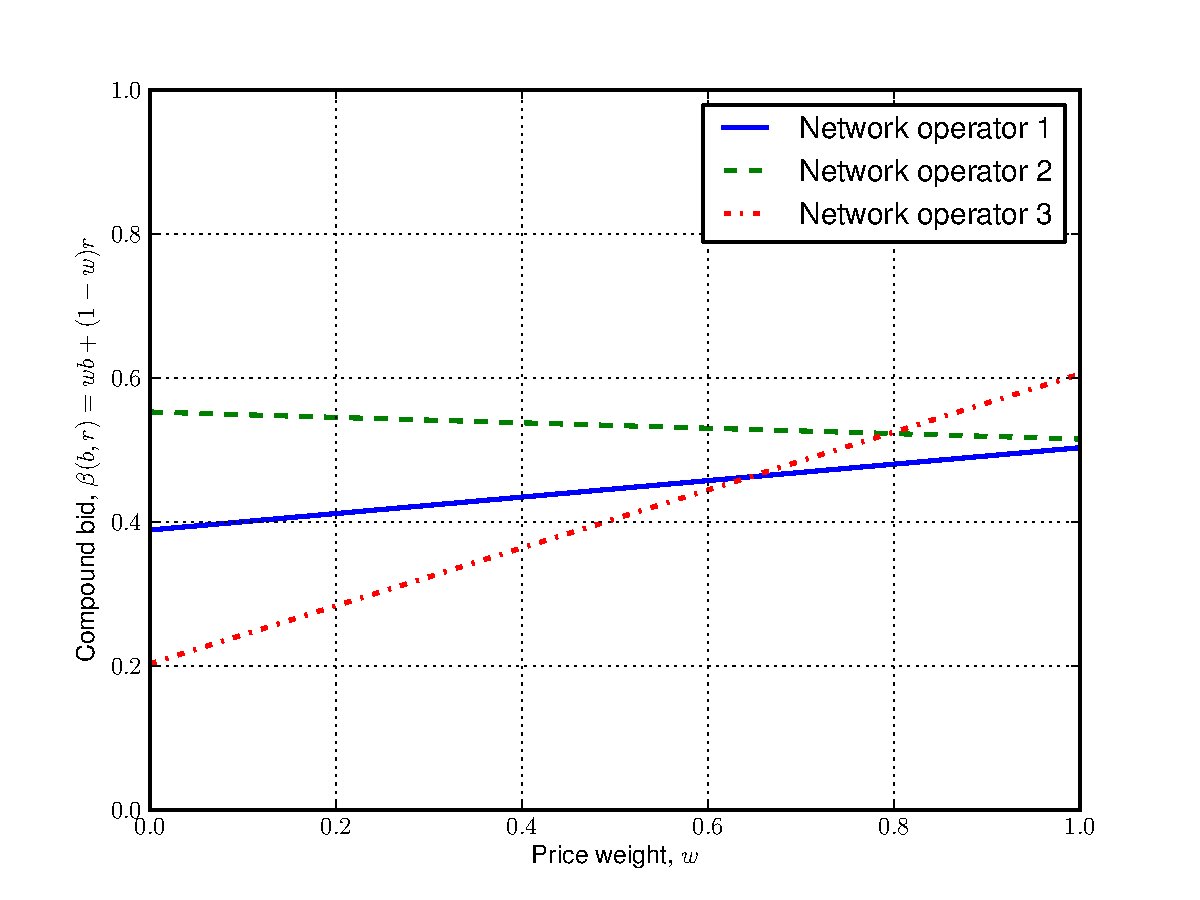
\includegraphics[width=\figsize]{Direct/Figures/bids_fpa}
	\caption{The performance of standard FPA bidding strategy, for the values of type, reputation and bid aggregated in Table~\ref{tab:bids_fpa_direct}}
	\label{fig:bids_fpa_direct}
\end{figure}

\begin{figure}[p!]
	\vspace{0.5cm}
	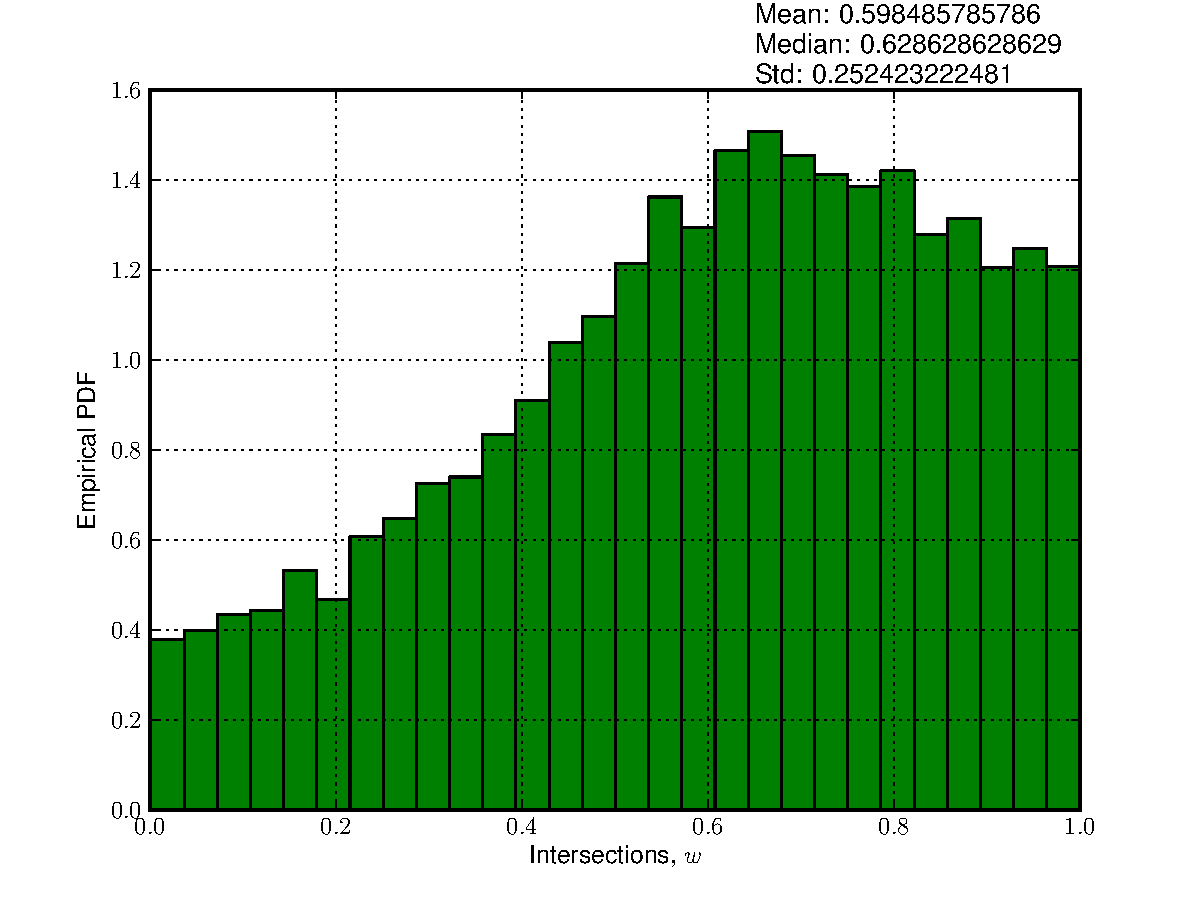
\includegraphics[width=\figsize]{Direct/Figures/hist_N_3}
	\caption{The empirical density function of the intersections (10,000 runs and 3 network operators)}
	\label{fig:hist_N_3_direct}
	\vspace{10mm}
	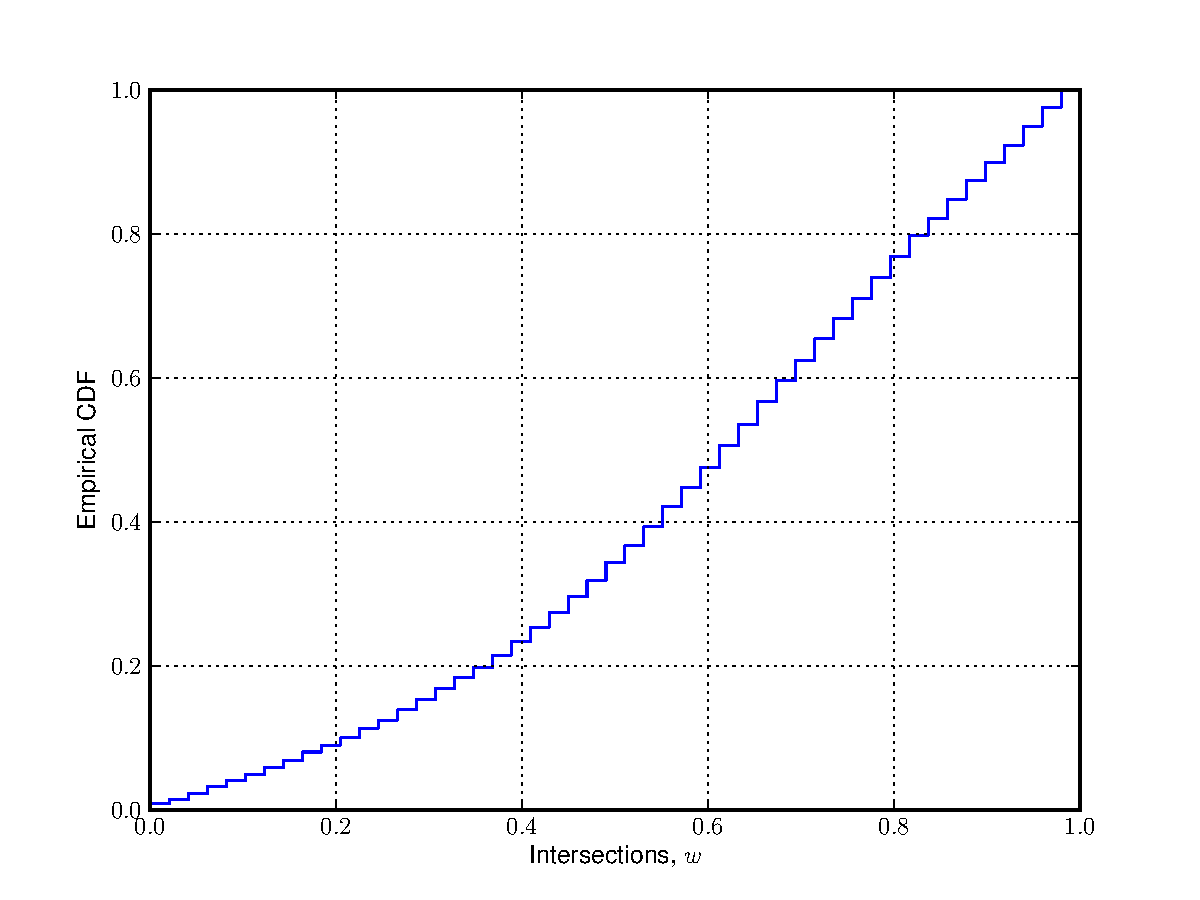
\includegraphics[width=\figsize]{Direct/Figures/ecdf_N_3}
	\caption{The empirical probability distribution associated with the histogram in Figure~\ref{fig:hist_N_3_direct}}
	\label{fig:ecdf_N_3_direct}
\end{figure}

Table~\ref{tab:bids_fpa_direct} and Figure~\ref{fig:bids_fpa_direct} depict a particular output from the simulation for $n=3$ network operators. In this particular example, for $w\in (0.65, 1]$, network operator 1 who is characterized by the lowest cost of all three network operators, wins the auction; that is, the network operator 1's compound bid is the lowest. At $w=0.65$, an intersection occurs of network operator 1's and 3's compound bids, and after that network operator 3 becomes the winner. If the simulation was repeated $r$ times, and the intersection was to fall within a close neighbourhood of $w=0.65$ in the vast majority of cases, then $b^*$ could quite likely be an equilibrium bidding strategy in the interval $w\in (0.65, 1]$. This is predicated on the fact that, as $w\rightarrow 1$, the offered price dominates the value of the compound bid; that is, the offered price is weighted more than the reputation rating (Equation~\eqref{eq:def_beta_direct}).

The methodology is as follows:
\begin{enumerate}
	\item Generate cost/reputation rating/bid triplet using the Monte Carlo methods.
	\item Find the winner for $w=1$, network operator $i$, say (in Figure~\ref{fig:bids_fpa_direct} that would be network operator~1).
	\item Decrease the value of $w$ until network operator $i$ no longer wins, and save the value of $w$ for which that happens. Henceforth, such an event shall be denoted by $I$, and called \emph{the event when an intersection has occurred.}
	\item If the intersection did not occur, $I=0$, increase the counter that counts the frequency of such an event, and then discard that run.
	\item Repeat $r$ number of times.
\end{enumerate}

The case when $r=10,000$ runs, and $n=3$ network operators is depicted in the two figures: Figure~\ref{fig:hist_N_3_direct} shows the empirical density function of the intersections; and Figure~\ref{fig:ecdf_N_3_direct} depicts the empirical distribution function of the intersections. The probability of an intersection occurring equals $P\{I=1\} = 0.67$. It can be concluded from the figures that, on average, intersections occur at $\bar{w}=0.6$, which represents the mean of the distribution. However, the peak observed in a close neighbourhood of $\bar{w}$ is not significant enough to conclude that bidding according to $b^*$ is the best strategy one can take for $w\in (\bar{w},1]$.

A more formal argument goes as follows. Figure~\ref{fig:ecdf_N_3_direct} depicts the probability that an intersection has occurred within an interval $(-\infty,w]$ given that an intersection has occurred, $I=1$; that is, if the former event is denoted by $W$, then the figure describes $P\{W\in(-\infty, w] \mid I=1\}$. From this, the probability of winning for network operator $i$ (as defined in the listing above) given any $w$ is
\begin{align}
	&P\{\text{winning} \mid w\} \nonumber\\
	&= 1 - P\{W\in[w,\infty) \cap I=1\} \nonumber\\
	&= 1 - P\{W\in[w,\infty)\mid I=1\}P\{I=1\} \nonumber\\
	&= 1 - \left( 1 - P\{W\in(-\infty, w]\mid I=1\} \right)P\{I=1\}.
	\label{eq:mc_prob_winning_direct}
\end{align}

In order to verify Equation~\eqref{eq:mc_prob_winning_direct}, let $w\in\{0.25,0.75\}$ and run a Monte Carlo simulation which counts the number of times when the network operator with the lowest cost is the winner; i.e., the winner of the auction for $w=1$. When $w=0.25$, 
\begin{equation*}
	P\{\text{winning}\mid w=0.25\} = 1 - (1-0.13)0.67 = 0.4171
\end{equation*}
according to Equation~\eqref{eq:mc_prob_winning_direct}, while the numerically obtained result 
\begin{equation*}
	P\{\text{winning}\mid w=0.25\} = 0.4136.
\end{equation*}
When $w=0.75$,
\begin{equation*}
	P\{\text{winning}\mid w=0.75\} = 1 -(1-0.68)0.67 = 0.7856
\end{equation*}
according to Equation~\eqref{eq:mc_prob_winning_direct}, while the numerically obtained result
\begin{equation*}
	P\{\text{winning}\mid w=0.75\} = 0.7866.
\end{equation*}

Clearly, the prediction based on Equation~\eqref{eq:mc_prob_winning_direct} converges to the numerically obtained result. Moreover, it is worth noting that for $w=0.25$, bidding according to $b^*$ guarantees the probability of winning for the network operator with the lowest cost of only $0.4171$ which is below $50\%$. Thus, the network operators will definitely deviate from $b^*$ for low values of $w$. On the other hand, for $w=0.75$, $b^*$ seems to achieve a relatively high probability of winning for the network operator with the lowest cost; i.e., the probability of $0.7856$. However, the argument is incomplete in the sense that it only considers the probability of winning rather than the expected utility.
% subsection special_case_w_1_ (end)

\subsection{Special Case $r_i=r_j$} % (fold)
\label{sub:special_case_r_i_r_j_direct}
In the last extreme case, when all network operators are characterized by the same reputation rating, i.e., when $r_i = r_j$ for all $i\neq j$, and when $w\neq 0$, it can be easily verified that the problem simplifies to the special case $w=1$. To see why, let $r = r_i,$ for all network operators $i$. Then, for all $i\in N$ and $w\neq 0$
\begin{align*}
	&\beta(b_i, r) < \min_{j\neq i} \beta(b_j, r)\\
	\iff &\frac{1}{w} \left(b_i + \frac{1-w}{w} r\right) < \frac{1}{w} \min_{j\neq i} \left(b_j + \frac{1-w}{w} r\right)\\
	\iff &b_i + \frac{1-w}{w} r < \min_{j\neq i} b_j + \frac{1-w}{w} r\\
	\iff &b_i < \min_{j\neq i} b_j.
\end{align*}
Hence, the utility of each network operator $i$ simplifies to
\begin{equation*}
	u_i(b,c,r) = \left\{
	\begin{array}{l l}
		b_i - c_i &\text{ if } b_i < \displaystyle\min_{j\neq i} b_j,\\
		0 &\text{ if } b_i > \displaystyle\min_{j\neq i} b_j.
	\end{array}
	\right.
\end{equation*}
Formally,
\begin{corollary}
\label{cor:special_case_r_i_r_j_direct}
Suppose $c_i$ is i.i.d.~over the interval $[0,1]$ for all $i\in N$ and $r_i\in [0,1]$ for all $i\in N$ is common knowledge. Suppose $r_i = r_j$ for all $i\neq j$, and $w\neq 0$. Then, the problem simplifies to the special case $w=1$, and hence, $b^*_{FPA}$ is the symmetric equilibrium bidding strategy (Proposition~\ref{prop:special_case_w_1_direct}).
\end{corollary}

In this section, we showed that, in the generic case, it is difficult to derive a closed-form solution to the bidding problem. Furthermore, we characerised the optimal bidding strategy in three special cases: $w=0$, $w=1$, $r_i=r_j$ for all $i,j\in N$ such that $i\neq j$.

The problem is considerably simplified by restricting the number of network operators to $n=2$, and letting the costs be drawn from the uniform distribution. In this case, it is possible to derive bidding strategies for both bidders, and this is the subject of the following section.
% subsection special_case_r_i_r_j_ (end)
% section generic_case (end)

\section{Restricted Case $n=2$} % (fold)
\label{sec:direct_restricted_case_n_2_direct}
In this section, we will restrict our attention to only two network operators. Since the problem in its generic form proved too complex to be solved analytically, this section will explore whether in a much simplified scenario it is possible to find a closed-form solution. To this end, let $n=2$. The utility function for each network operator $i\in N$ thus becomes
\begin{equation}
	\label{eq:utility_n_2_direct}
	u_i(b,c,r) = \left\{
	\begin{array}{l l}
		b_i - c_i &\text{if } \beta(b_i,r_i) < \beta(b_j,r_j),\\
		\frac{1}{2}(b_i - c_i) &\text{if } \beta(b_i,r_i) = \beta(b_j,r_j),\\
		0 &\text{otherwise}.
	\end{array}\right.
\end{equation}
Furthermore, the assumption concerning the symmetric equilibrium profile is relaxed; that is, network operators are permitted to use differing bidding strategies.

The analysis is conducted in two steps. Firstly, it is assumed that information is complete; that is, that each network operator not only knows their own cost and reputation, but also those of their opponent's. Secondly, the standard case is considered; that is, that the reputation ratings of the network operators are assumed to be known, while the costs are private knowledge.

\subsection{Complete Information} % (fold)
\label{sub:complete_information_n_2_direct}
Here, we assume that information is complete; i.e., that each network operator knows their own and their opponent's cost and reputation rating. In total, there are 7 different bidding scenarios to consider as described below.

\begin{figure}[p!]
	\vspace{0.5cm}
	\begin{subfigure}[b]{0.5\textwidth}
	  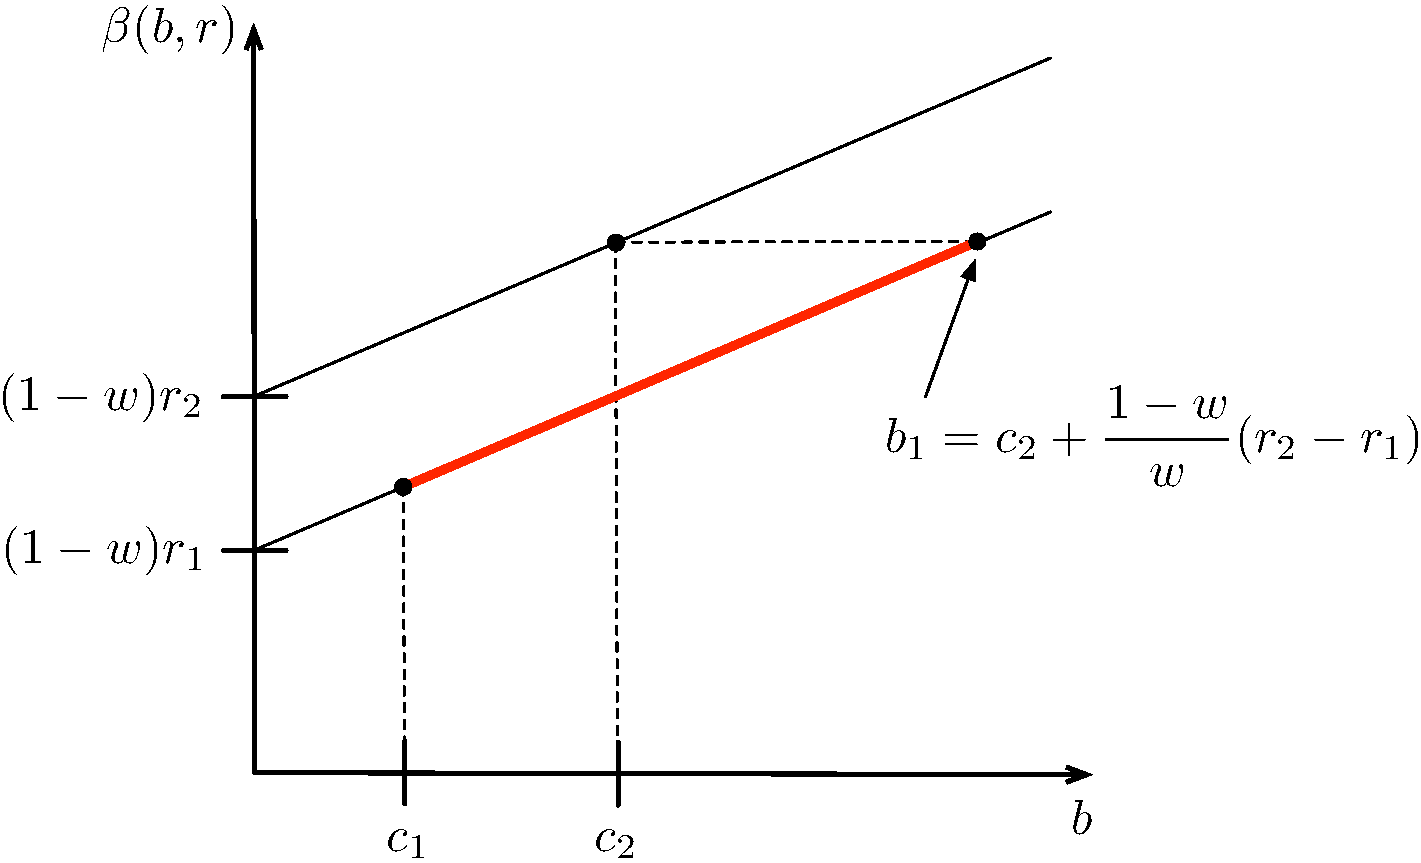
\includegraphics[width=2.8in]{Direct/Figures/complete_N_2_c1}
	  \caption{$c_i < c_j$}
	  \label{fig:complete_N_2_c1_direct}
	\end{subfigure}
	\begin{subfigure}[b]{0.5\textwidth}
	  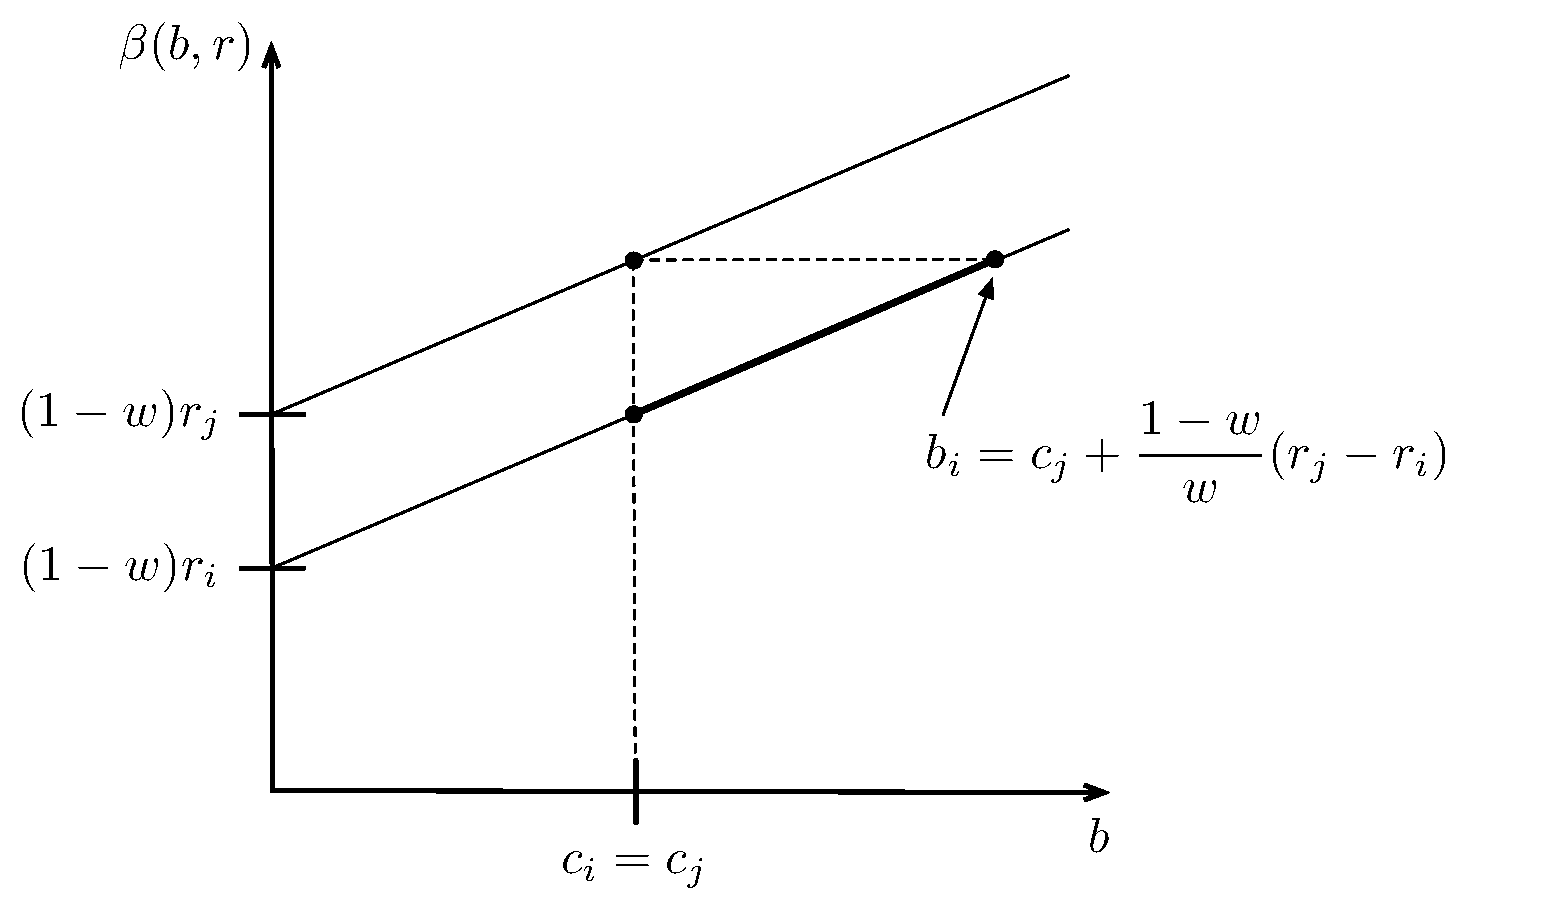
\includegraphics[width=2.8in]{Direct/Figures/complete_N_2_c2}
	  \caption{$c_i = c_j$}
	  \label{fig:complete_N_2_c2_direct}
	\end{subfigure}
	\vspace{0.5cm}\\
	\begin{subfigure}[b]{0.5\textwidth}
	  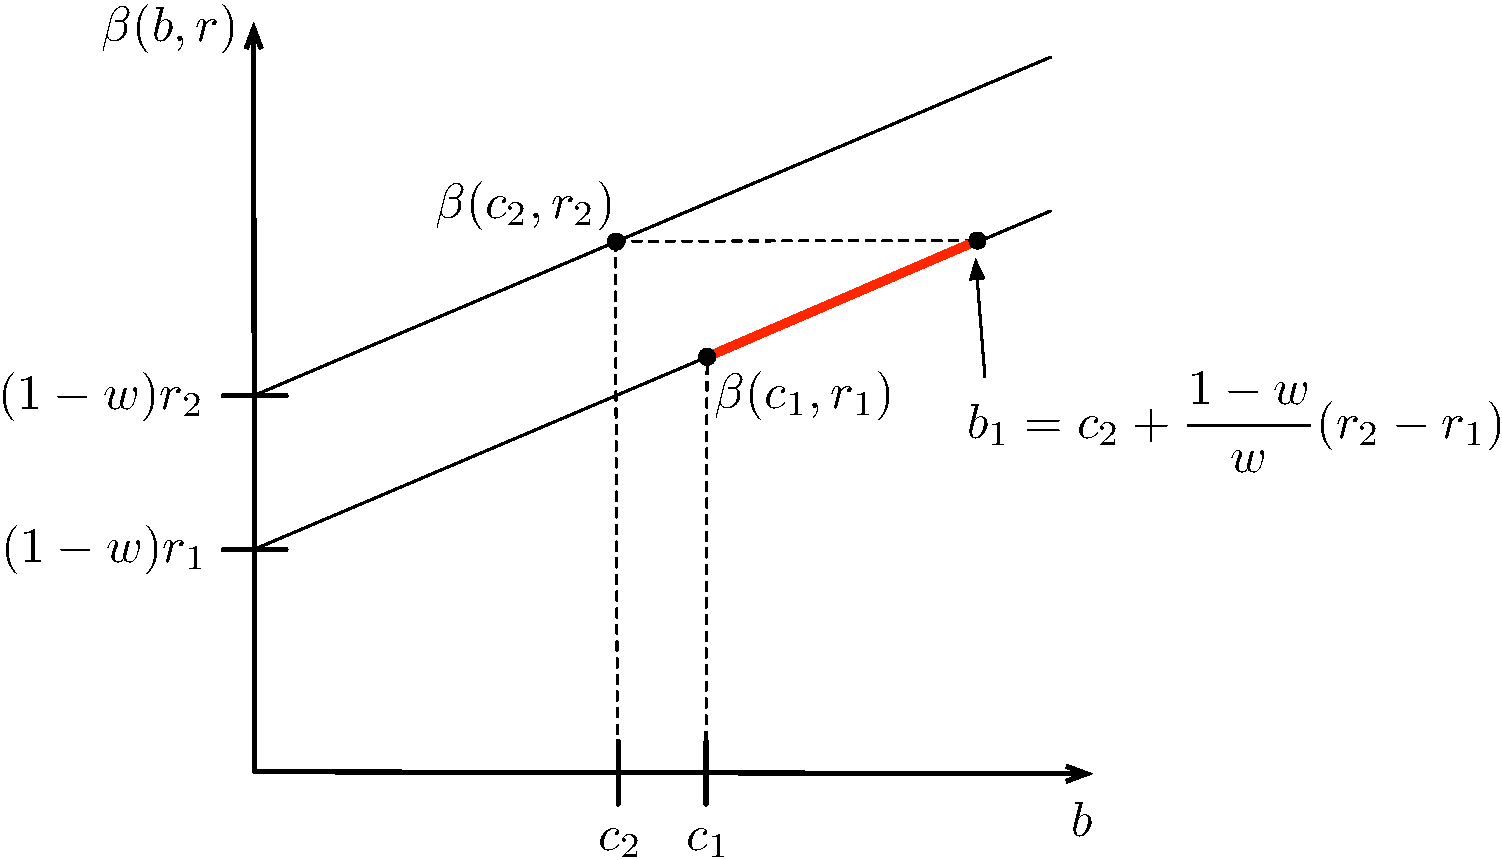
\includegraphics[width=2.8in]{Direct/Figures/complete_N_2_c3_1}
	  \caption{$c_i > c_j$ and $\beta(c_i,r_i) < \beta(c_j,r_j)$}
	  \label{fig:complete_N_2_c3_1_direct}
	\end{subfigure}
	\begin{subfigure}[b]{0.5\textwidth}
	  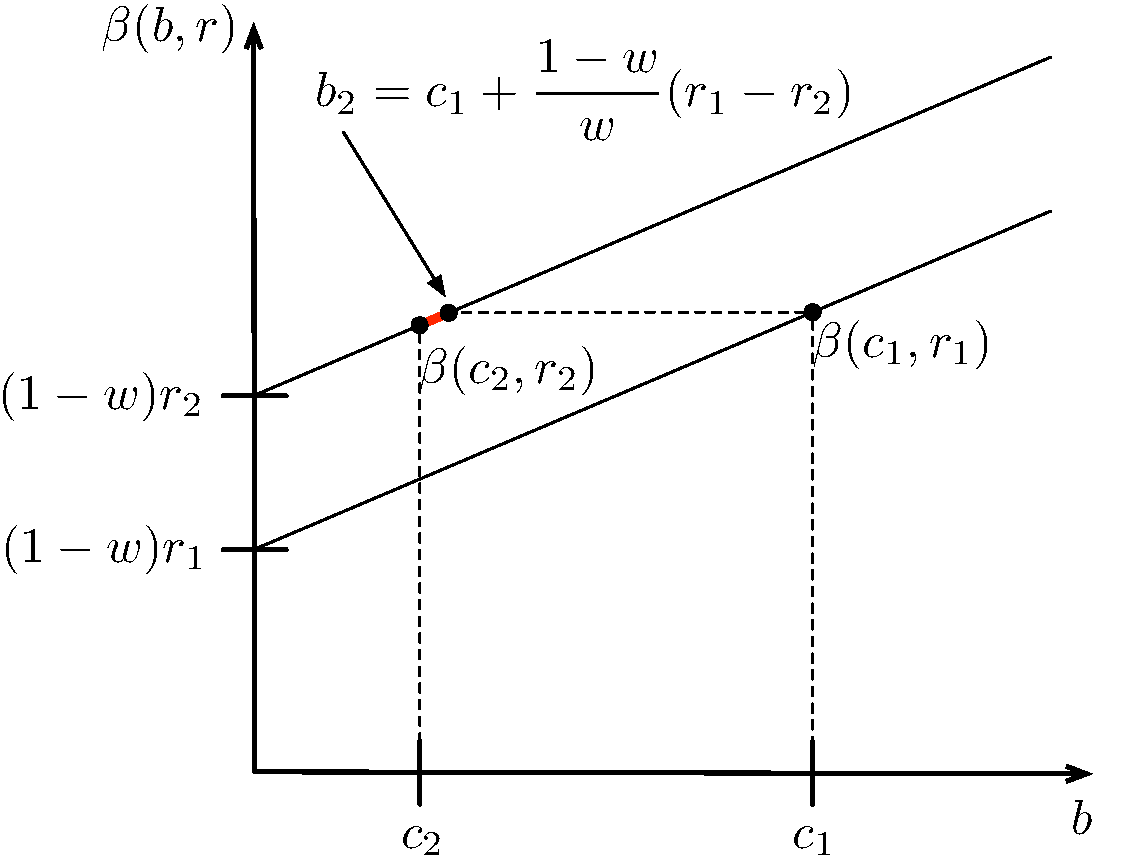
\includegraphics[width=2.8in]{Direct/Figures/complete_N_2_c3_2}
	  \caption{$c_i > c_j$ and $\beta(c_i,r_i) \ge \beta(c_j,r_j)$}
	  \label{fig:complete_N_2_c3_2_direct}
	\end{subfigure}
	\caption{Different bidding scenarios for $r_i < r_j$}
	\label{fig:complete_N_2_1_direct}
\end{figure}

\begin{figure}[p!]
	\vspace{0.5cm}
	\begin{subfigure}[b]{0.5\textwidth}
		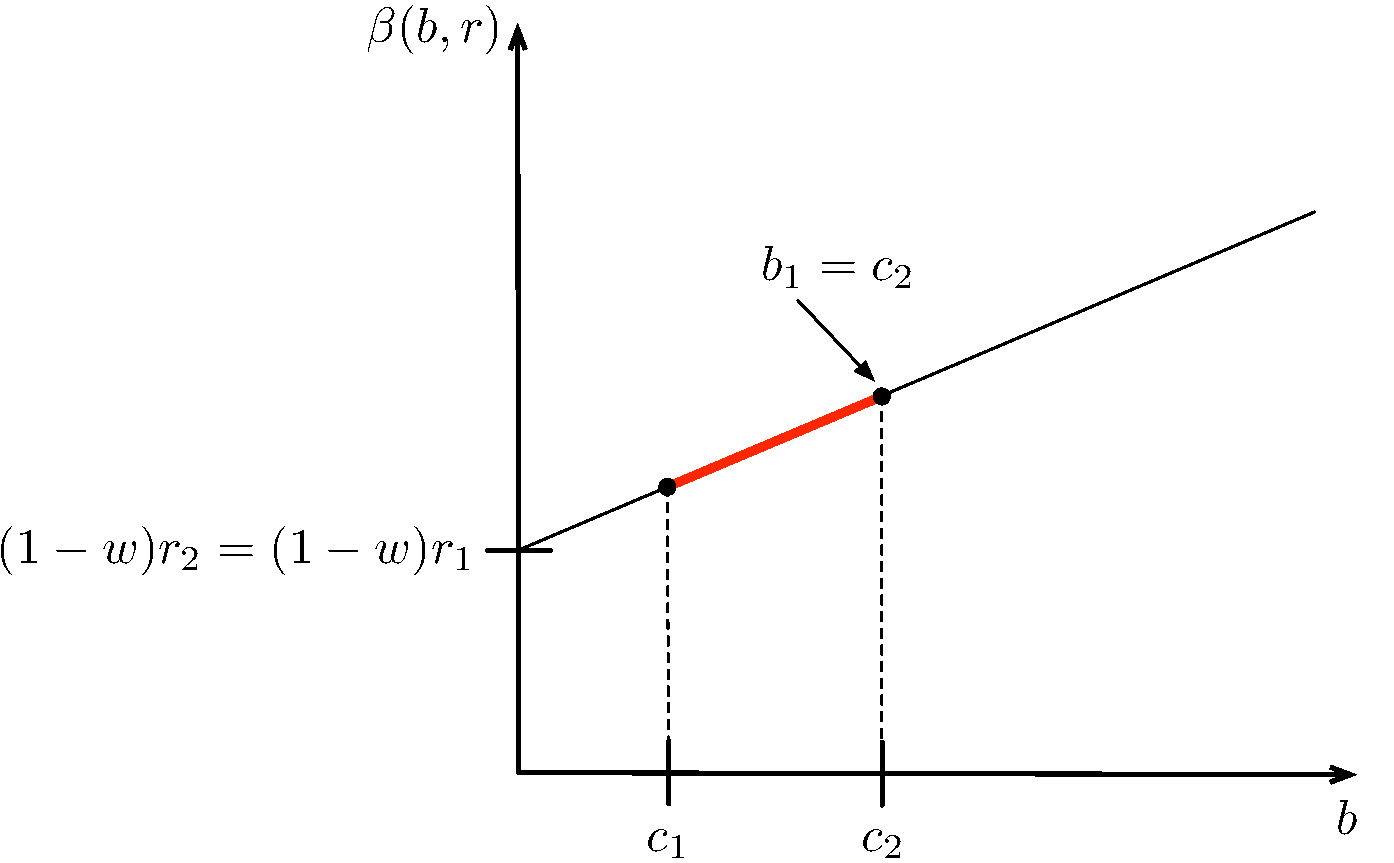
\includegraphics[width=2.8in]{Direct/Figures/complete_N_2_c4}	  
	  \caption{$c_i<c_j$}
	  \label{fig:complete_N_2_c4_direct}
	\end{subfigure}
	\vspace{0.5cm}\\
	\begin{subfigure}[b]{0.5\textwidth}
	  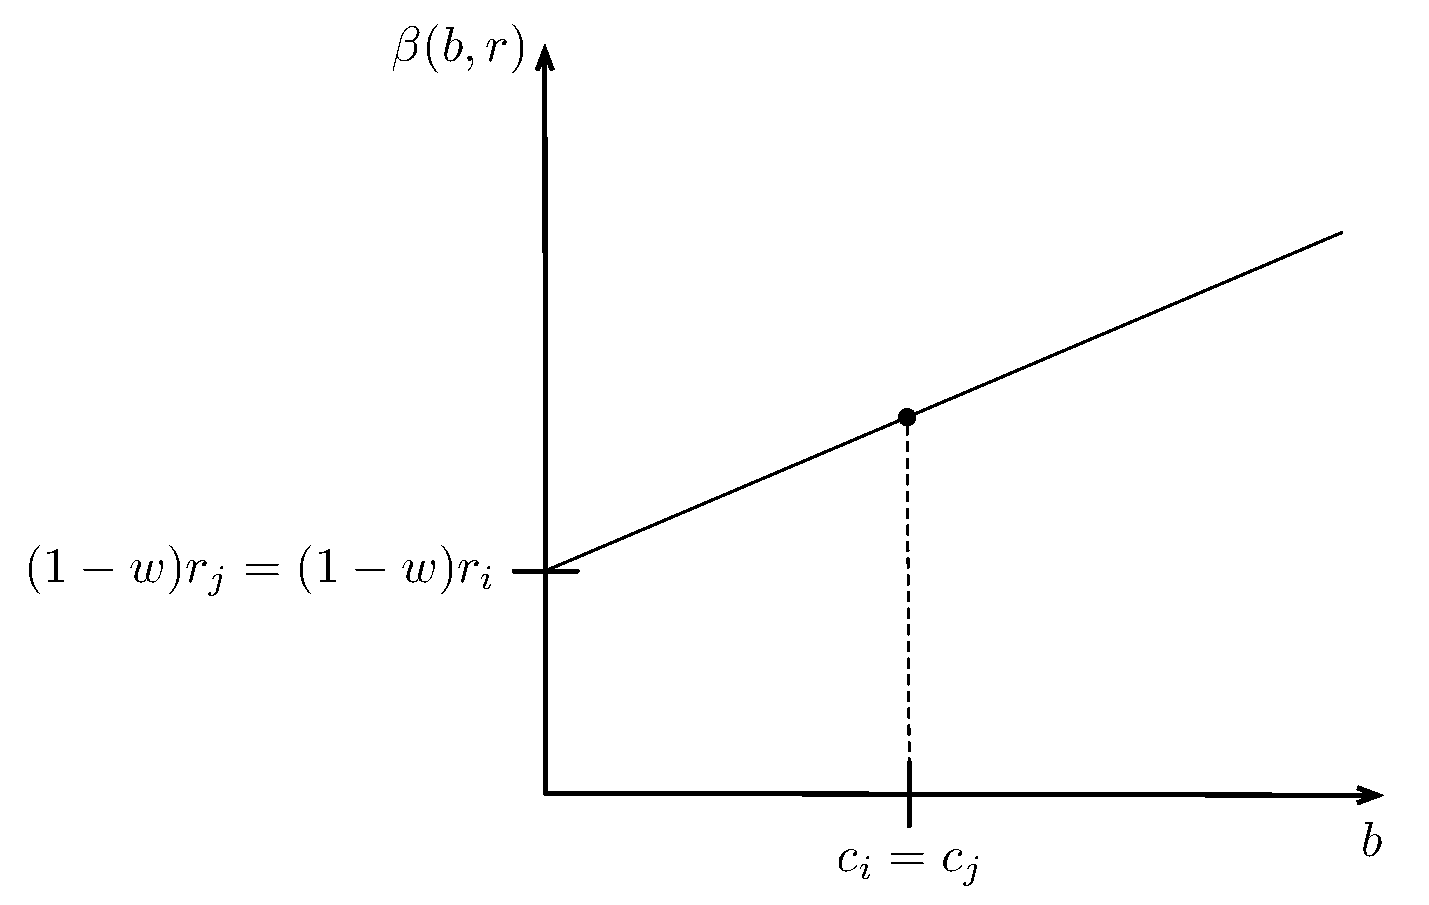
\includegraphics[width=2.8in]{Direct/Figures/complete_N_2_c5}
	  \caption{$c_i=c_j$}
	  \label{fig:complete_N_2_c5_direct}
	\end{subfigure}
	\vspace{0.5cm}\\
	\begin{subfigure}[b]{0.5\textwidth}
	  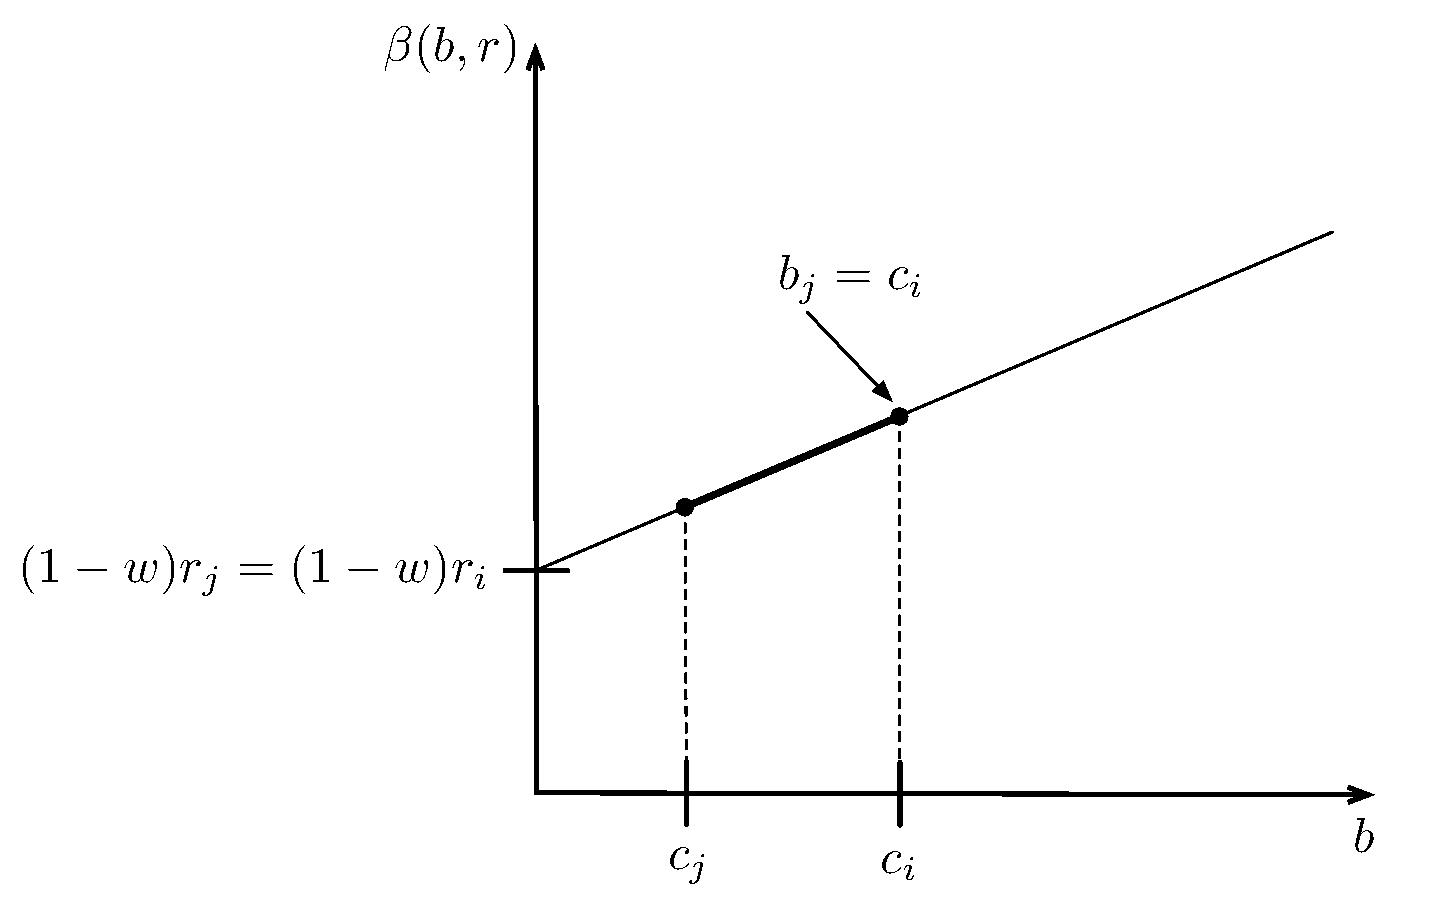
\includegraphics[width=2.8in]{Direct/Figures/complete_N_2_c6}
	  \caption{$c_i > c_j$}
	  \label{fig:complete_N_2_c6_direct}
	\end{subfigure}
	\caption{Different bidding scenarios for $r_i = r_j$}
	\label{fig:complete_N_2_2_direct}
\end{figure}

Figure~\ref{fig:complete_N_2_1_direct} shows the first 4 cases for which $r_i < r_j$. (Note that exactly the same reasoning applies to the situation when $r_i > r_j$.) If $c_i < c_j$, network operator $i$ is guaranteed a victory and a positive profit as long as they bid within the highlighted part of the $\beta(b,r)$ curve depicted in Figure~\ref{fig:complete_N_2_c1_direct}. Thus, their optimal bidding strategy would be to bid slightly less than their opponent's compound bid evaluated at their opponent's cost, $\beta(c_j,r_j)$; that is, $b_i = c_j + \frac{1-w}{w}(r_j-r_i) - \epsilon$ where $\epsilon>0$ is very small. Network operator $j$, on the other hand, should find it optimal to bid $b_j = c_j$. To see why, suppose network operator $j$ bids $\hat{b}_j>c_j$. Since network operator $i$'s reputation rating and cost are strictly lower than those of network operator $j$'s, they can undercut the network operator $j$'s bid by a small amount so that $\hat{b}_i < \hat{b}_j$ and still make positive profit. But, in response, network operator $j$ will find it optimal to lower their bid so that it undercuts that of network operator $i$'s; that is, $\hat{b}_j < \hat{b}_i$. This process will continue until one of the network operators is forced to bid their cost. Since network operator $i$'s reputation rating and cost are strictly lower than those of network operator $j$'s, we conclude that $b_j = c_j$ and $b_i = c_j + \frac{1-w}{w}(r_j-r_i) - \epsilon$ where $\epsilon>0$ is very small.

If $c_i = c_j$, arguing in the similar manner as previously, network operator $i$'s optimal bidding strategy would be to bid $b_i = c_j + \frac{1-w}{w}(r_j-r_i) - \epsilon$ where $\epsilon>0$ is very small; while network operator $j$ should bid $b_j = c_j$ (Figure~\ref{fig:complete_N_2_c2_direct}).

If $c_i > c_j$, there are two cases to consider. If $\beta(c_i,r_i)<\beta(c_j,r_j)$, then network operator $i$ still has some room for manoeuvre, and should find it optimal to bid $b_i = c_j + \frac{1-w}{w}(r_j-r_i) - \epsilon$ where $\epsilon>0$ is very small; while network operator $j$ to bid $b_j=c_j$ (Figure~\ref{fig:complete_N_2_c3_1_direct}). If $\beta(c_i,r_i)\ge \beta(c_j,r_j)$, on the other hand, the roles are reversed, and network operator $j$ should find it optimal to bid $b_j = c_i + \frac{1-w}{w}(r_i-r_j) - \epsilon$ where $\epsilon>0$ is very small; while network operator $i$ to bid $b_i = c_i$ (Figure~\ref{fig:complete_N_2_c3_2_direct}).

Figure~\ref{fig:complete_N_2_2_direct} depicts the remaining 3 cases for which $r_i=r_j$. If $c_i < c_j$, network operator $i$'s optimal bidding strategy would be to bid $b_i = c_j - \epsilon$ where $\epsilon>0$ is very small; while network operator $j$ should bid $b_j = c_j$ (Figure~\ref{fig:complete_N_2_c4_direct}).

If $c_i = c_j$, both network operators should bid their costs; that is, $b_i = c_i$ and $b_j = c_j$ (Figure~\ref{fig:complete_N_2_c5_direct}).

If $c_i > c_j$, network operator $j$'s optimal bidding strategy would be to bid $b_j = c_i - \epsilon$ where $\epsilon>0$ is very small; while network operator $i$ should bid $b_i = c_i$ (Figure~\ref{fig:complete_N_2_c6_direct}).

It can be concluded that the bidding strategies depend only on costs if $r_i = r_j$. In the remaining cases, they are asymmetric in the sense that the winning network operator is characterized by
\begin{equation*}
	b_i = c_j + \frac{1-w}{w}(r_j - r_i) - \epsilon \quad\text{with }\epsilon>0\text{ being very small},
\end{equation*}
while the losing network operator by bidding their own cost
\begin{equation*}
	b_j = c_j.
\end{equation*}
Hence, when dealing with incomplete information, we will exploit these results by concentrating on equilibrium bidding strategies which are linear functions of cost.
% subsection complete_information_n_2 (end)

\subsection{Incomplete Information} % (fold)
\label{sub:incomplete_information_n_2_direct}
Here, contrary to previous section, we assume the standard case; that is, that reputation rating values for both network operators are known at the time of bidding; however, their costs are private knowledge. Suppose that the network operators use a strategy function $b_i: [0,1]\to\mathbb{R}$ defined by the rule
\begin{equation}
	\label{eq:pcomp_bidding_str_direct}
	b_i(c_i) = m_i + n_i c_i,\quad\text{for all } m_i\in\mathbb{R},n_i>0,
\end{equation}
and costs are independently drawn from the uniform distribution over the interval $[0,1]$. In other words, (although somewhat counter-intuitive) we allow for negative bids from the network operators. The motivation for such an assumption will be explained in detail later on in the section. Note, moreover, that the strategy function is assumed to be linear in cost. Each network operator $i$ faces an optimization problem
\begin{equation}
	\label{eq:pcomp_exp_utility_uc_direct}
	\max_{b_i}E \left[ b_i-c_i \:\middle\vert\: wb_i + (1-w)r_i < w(m_j + n_j C_j) + (1-w)r_j\right]
\end{equation}

If $w=0$, then the result described in Proposition~\ref{prop:special_case_w_0_direct}, Section~\ref{sub:special_case_w_0_direct}, holds. Otherwise, for $0<w\le 1$, each network operator $i$ solves
\begin{align}
	&\max_{b_i} E \left[ b_i-c_i \:\middle\vert\: \frac{1}{n_j}\left( b_i + \frac{1-w}{w}(r_i-r_j)-m_j \right) < C_j \right] \nonumber\\
	= &\max_{b_i}\int_{\frac{1}{n_j}(b_i + \frac{1-w}{w}(r_i-r_j)-m_j)}^{1} (b_i-c_i)dF_C(t)\nonumber\\
	= &\max_{b_i} \bigg(b_i-c_i\bigg) \left(1-\frac{1}{n_j}b_i-\frac{1}{n_j} \left(\frac{1-w}{w}(r_i-r_j)-m_j \right) \right).
	\label{eq:pcomp_exp_utility_w_1_direct}
\end{align}
The first-order condition yields
\begin{align}
	&\qquad\quad 1 - \frac{2}{n_j}b_i + \frac{1}{n_j}c_i - \frac{1}{n_j}\left( \frac{1-w}{w}(r_i-r_j) - m_j \right) = 0 \nonumber\\
	&\iff b_i = \frac{n_j}{2} - \frac{1}{2}\left( \frac{1-w}{w}(r_i-r_j) - m_j \right) + \frac{1}{2}c_i.
\end{align}
(Note that the second-order condition is satisfied; i.e., $\frac{d^2}{db^2_i}E[\cdot\vert\cdot] = -\frac{2}{n_j} < 0$ since $n_j>0$.) Similar argument for network operator $j$ yields
\begin{equation}
	b_j = \frac{n_i}{2} - \frac{1}{2}\left( \frac{1-w}{w}(r_j-r_i) - m_i \right) + \frac{1}{2}c_j.
\end{equation}
Thus, it follows
\begin{equation*}
	\left\{
	\begin{array}{l l}
		n_i &= n_j = \displaystyle\frac{1}{2},\\[2ex]
		m_i &= \displaystyle\frac{n_j}{2} - \displaystyle\frac{1}{2}\left( \displaystyle\frac{1-w}{w}(r_i-r_j) - m_j \right),\\[2ex]
		m_j &= \displaystyle\frac{n_i}{2} - \displaystyle\frac{1}{2}\left( \displaystyle\frac{1-w}{w}(r_j-r_i) - m_i \right).
	\end{array}\right.
\end{equation*}
Solving the above equations simultaneously yields the equilibrium bidding strategy,
\begin{equation*}
	b_i'(c_i) = \frac{1}{2} - \frac{1-w}{3w}(r_i-r_j) + \frac{1}{2}c_i \quad\text{for all } i\in N.
\end{equation*}
Formally,
\begin{proposition}
\label{prop:pcomp_equi_bidding_str_direct}
Let there be $n=2$ network operators. Suppose $c_i$ is independently drawn from uniform distribution over the interval $[0,1]$ for all $i\in N$, and $r_i\in [0,1]$ for all $i\in N$ is common knowledge. Then the equilibrium bidding strategy for all $w\in (0,1]$ is given by
\begin{equation}
	\label{eq:pcomp_equi_bidding_str_direct}
	b_i'(c_i) = \frac{1}{2} - \frac{1-w}{3w}(r_i-r_j) + \frac{1}{2}c_i.
\end{equation}
\end{proposition}
\noindent Observe that the pair of strategies $(b_i', b_j')$ does not constitute a symmetric equilibrium.

\begin{table}[h]
	\caption{An exemplary set of cost-reputation pairs of two network operators}
	\vspace{0.5cm}
	\begin{tabular*}{0.5\columnwidth}[L]{@{\extracolsep{\fill}}r c c}
		\hlx{vhv}
		& \textbf{Cost}, $c_i$ & \textbf{Reputation rating}, $r_i$\\
		\hlx{vhv}
		\textbf{Network operator 1} & $0.75$ & $0.25$\\
		\textbf{Network operator 2} & $0.25$ & $0.75$\\
		\hlx{vhs}
	\end{tabular*}
	\label{tab:pcomp_direct}
\end{table}

\begin{figure}[p!]
	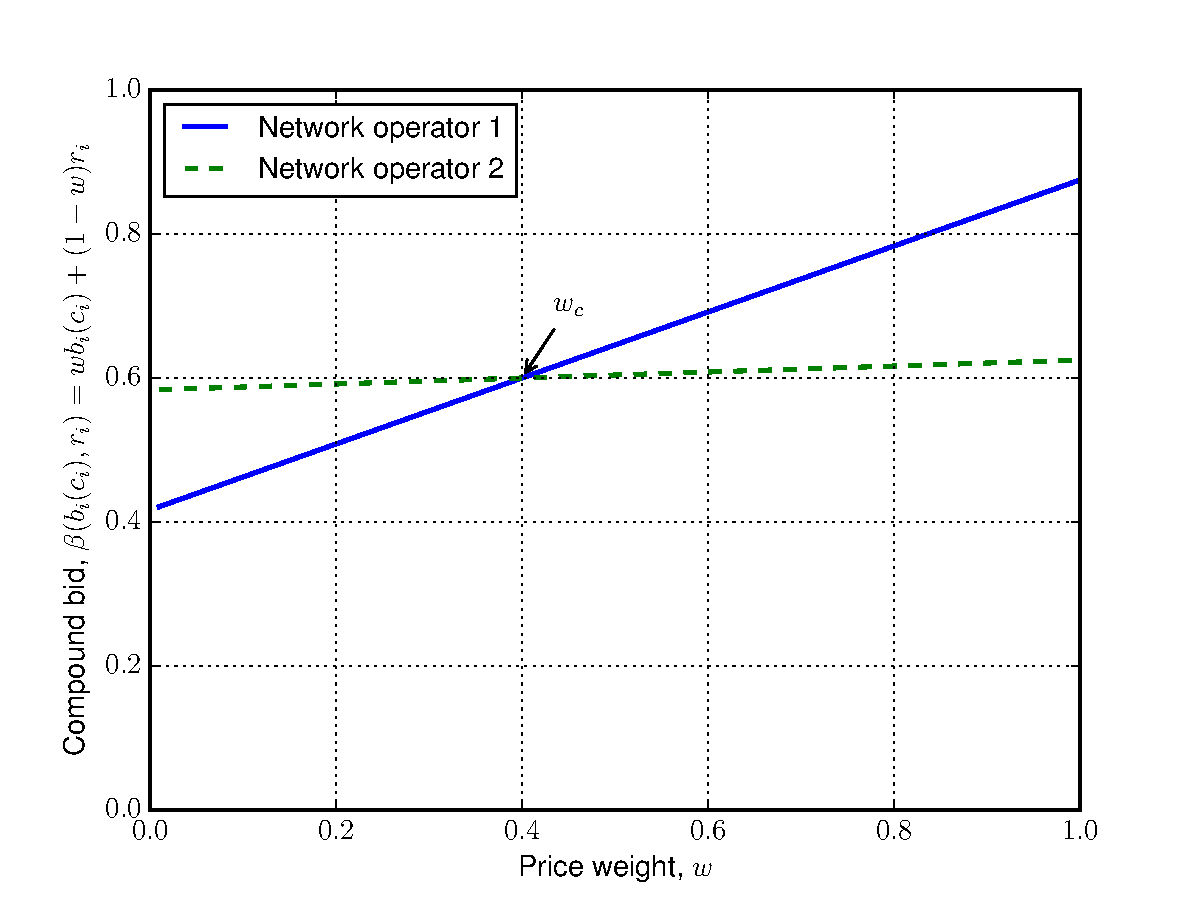
\includegraphics[width=\figsize]{Direct/Figures/pincomplete_bids_uc}
	\caption{Compound bid plotted against the price weight}
	\label{fig:pincomplete_bids_uc_direct}
	\vspace{10mm}
	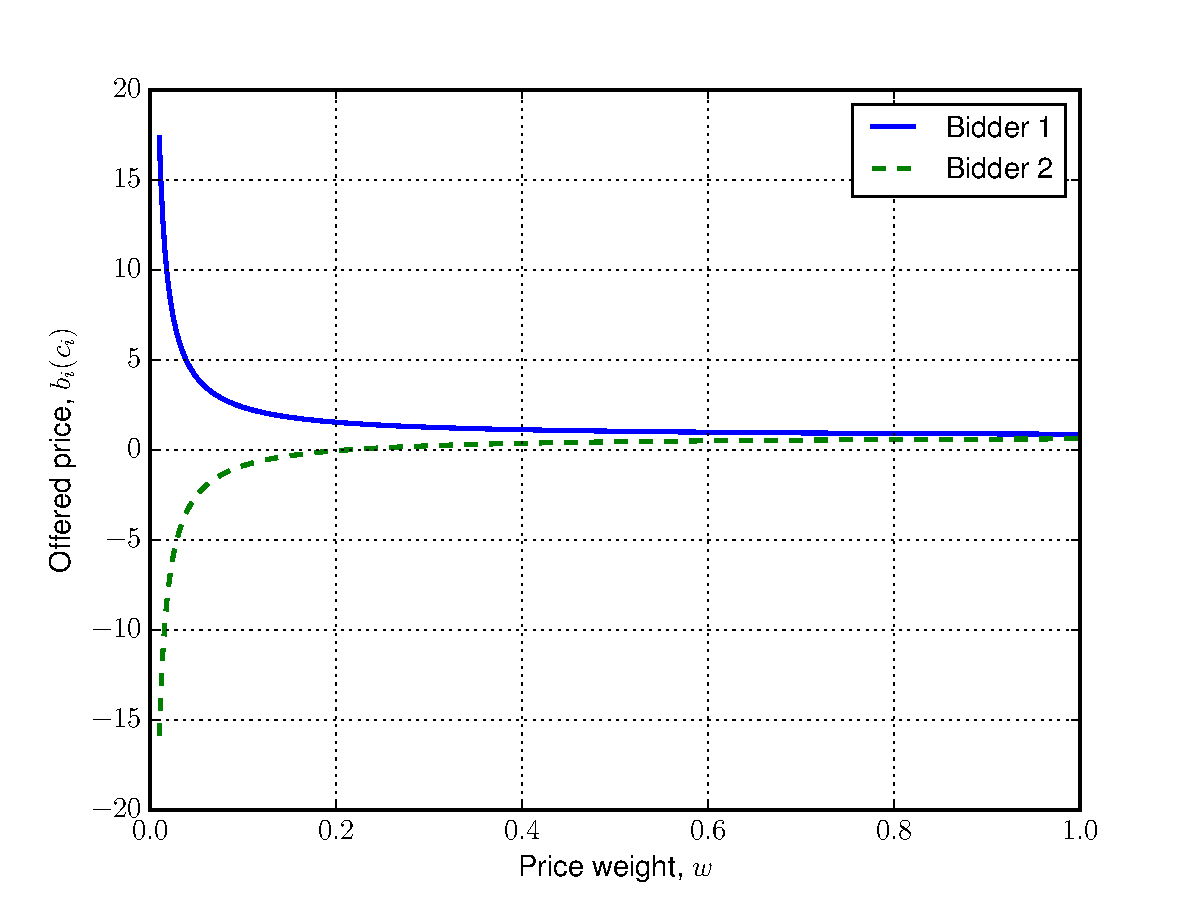
\includegraphics[width=\figsize]{Direct/Figures/pincomplete_prices_uc}
	\caption{Offered prices (bids) plotted against the price weight}
	\label{fig:pincomplete_prices_uc_direct}
\end{figure}

By way of example, Table~\ref{tab:pcomp_direct} depicts a particular set of cost-reputation pairs of two network operators. Figure~\ref{fig:pincomplete_bids_uc_direct} shows the value of the compound bid, $\beta$, for different values of $w$ for both network operators, while Figure~\ref{fig:pincomplete_prices_uc_direct} depicts the value of the monetary bid (or offered price), $b'_i$, for different values of $w$ for both network operators. The numerical data in Table~\ref{tab:pcomp_direct} suggests that network operator 2 should be the winner for the values of $w\rightarrow 1$ since network operator 2's cost is strictly lower than that of their opponent's. On the other hand, network operator 1 should be winner for the values of $w\rightarrow 0$ since network operator 1's reputation rating is strictly lower than that of their opponent's (which implies that network operator 1's reputation is in fact strictly higher than that of their opponent's). This prediction agrees with the numerical output shown in Figure~\ref{fig:pincomplete_bids_uc_direct}. Let $w_c$ denote the value of $w$ for which an intersection between the compound bids of both network operators occurs (if it exists). In Figure~\ref{fig:pincomplete_bids_uc_direct}, $w_c=0.4$. Hence, network operator 2 wins the auction for the values of $w\in(w_c,1]$, while network operator 1 for the values of $w\in[0,w_c)$. Note, moreover, that network operator 2 bids below their cost for values of $w<w_c$ (Figure~\ref{fig:pincomplete_prices_uc_direct}). However, this does not necessarily disqualify the equilibrium bidding strategies given by Equation~\eqref{eq:pcomp_equi_bidding_str_direct}. The following observations show why. Firstly,
\begin{proposition}
\label{prop:pcomp_negative_bids_direct}
Suppose both network operators bid according to $b_i'$ bidding strategies. Then they are guaranteed nonnegative profit in case of winning (or a draw).
\end{proposition}
\noindent Even though the prediction suggests that one of the network operators may bid negatively, they will not win the auction, and hence, are guaranteed profit at worst equal to zero.

Secondly, let $(\mathbf{Q},\mathbf{M})$ be the direct mechanism induced by the equilibrium bidding strategies, $b_i'$, in Equation~\eqref{eq:pcomp_equi_bidding_str_direct} where $\mathbf{Q}=(Q_i,Q_j)$ and $\mathbf{M}=(M_i,M_j)$. Here, $Q_i$ represents the allocation rule defined by
\begin{equation}
	\label{eq:pcomp_allocation_rule_direct}
	Q_i(c_i,c_j) =
	\left\{
	\begin{array}{l l}
		1 &\text{if } \beta(b_i'(c_i),r_i) < \beta(b_j'(c_j),r_j)\\
		\frac{1}{2} &\text{if } \beta(b_i'(c_i),r_i) = \beta(b_j'(c_j),r_j)\\
		0 &\text{otherwise}
	\end{array}
	\right.,
\end{equation}
while $M_i$ is the payment rule defined by
\begin{equation}
	\label{eq:pcomp_payment_rule_direct}
	M_i(c_i,c_j) = Q_i(c_i,c_j)b_i'(c_i).
\end{equation}
Suppose network operator $j$ reveals their cost truthfully. The equilibrium payoff function for network operator $i$ characterized by cost $c_i$ but revealing $c'_i$ is
\begin{align}
	\tilde{\tilde{u}}_i(c'_i) &= E\left[ M_i(c'_i,C_j) - c_iQ_i(c'_i,C_j) \right]\nonumber \\
	&= E\left[ (b_i'(c'_i)-c_i)Q_i(c'_i,C_j) \right]\nonumber \\
	&= E\left[ b_i'(c'_i)-c_i \:\middle\vert\: \beta(b_i'(c'_i),r_i) < \beta(b_j'(C_j),r_j) \right].
	\label{eq:pcomp_expected_utility_direct}
\end{align}
It turns out that it is in network operator $i$'s best interest to reveal their cost truthfully as well; i.e., $c'_i=c_i$. Moreover, both network operators cannot be better off by not participating in the auction; i.e., their equilibrium payoff function is nonnegative, $\tilde{\tilde{u}}_i(c_i)\ge 0$. Formally,
\begin{proposition}
\label{prop:pcomp_direct_mechanism_direct}
The direct mechanism $(\mathbf{Q},\mathbf{M})$ where $\mathbf{Q}=(Q_i,Q_j)$ and $\mathbf{M}=(M_i,M_j)$ (with $Q_i$ and $M_i$ defined in Equations~\eqref{eq:pcomp_allocation_rule_direct} and \eqref{eq:pcomp_payment_rule_direct} respectively) satisfies both the IC and IR constraints.
\end{proposition}

Thirdly, suppose that economic agents are computers who bid on behalf of the network operators. This assumption is reasonable since there currently are estimated 6.1 billion mobile subscribers around the world \cite{Ericsson2011}. In other words, bidding on a per call basis would have to be automated by the network operators in order to make the process manageable. One way of achieving such an automation would be to utilise the concept of a direct mechanism. In a direct mechanism, economic agents submit their costs (which need not be truthful) directly to the mechanism which then computes the bids and chooses the winner on their behalf. By the Revelation Principle\footnote{See Apendix~\ref{cha:notation} for the definition of the Revelation Principle.}, we know that for every mechanism and an equilibrium for that mechanism, there exists an incentive compatible direct mechanism which yields the same outcomes as in the given equilibrium of the original mechanism. In our case, the direct mechanism $(\mathbf{Q},\mathbf{M})$ is the direct representation of the DMP variant of an FPA. Since it is incentive compatible, economic agents will not lie about their costs. Since it is individually rational, they will find it beneficial to participate in the mechanism. Therefore, the possibility of one of the network operators bidding below their cost or negatively will not matter to any of the network operators and will not lead to an outcome in which the service is sold for a negative price.

Nonetheless, the possibility of one of the network operators bidding below their cost or negatively might seem counter-intuitive and irrational. The most straightforward solution is to constrain the original optimization problem in Equation~\eqref{eq:pcomp_exp_utility_uc_direct}; that is, each network operator $i$ tries to solve for all $w\neq 0$
\begin{align}
	\label{eq:pcomp_exp_utility_c_direct}
	&\max_{b_i}E \left[ b_i-c_i \:\middle\vert\: wb_i + (1-w)r_i < w(m_j + n_j C_j) + (1-w)r_j\right]\\
	&\text{subject to}\quad c_i-b_i\le 0.\nonumber
\end{align}
The constraint $c_i-b_i\le 0$ ensures that each network operator bids above or equal to their cost. However, this problem is much more complicated than its unconstrained version in Equation~\eqref{eq:pcomp_exp_utility_uc_direct}. Not only is it necessary to solve the nonlinear constrained optimization problem for each network operator $i$, but also it needs to be done simultaneously \cite{Griffin2011}. To better explore the inherent complexity of the problem, we will apply the Karush-Kuhn-Tucker Conditions theorem\footnote{See Appendix~\ref{cha:notation} for the definition of the Karush-Kuhn-Tucker Conditions theorem.}, and try to derive the equilibrium bidding strategies for all network operators. But first, note that, since $n_j>0$ ($n_i>0$ for network operator $j$), $E[\cdot \vert \cdot]$ is a concave function of $b_i$ ($b_j$ for network operator $j$). Moreover, the constraint as a function of $b_i$ ($b_j$ for network operator $j$) is affine, and hence convex. Therefore, the Karush-Kuhn-Tucker Conditions are necessary and sufficient conditions for a solution in nonlinear constrained optimization problem to be optimal.

The problem will be approached as follows. First, we will fix the bidding strategy for network operator $j$ and treat the problem as a standard nonlinear constrained optimization problem for network operator $i$. The same stage will be repeated for network operator $j$. Then the results of both stages will be combined together and solved simultaneously. In effect, this will result in derivation of the equilibrium bidding strategies for both network operators.

The Lagrangian of the problem for network operator $i$ is
\begin{align}
	&L_i(b_i,\lambda_i) \nonumber\\
	&= E \left[ b_i-c_i \:\middle\vert\: wb_i + (1-w)r_i < w(m_j + n_j C_j) + (1-w)r_j\right] - \lambda_i(c_i-b_i) \nonumber\\
	&= (b_i-c_i)\left(1-\frac{1}{n_j}b_i - \frac{1}{n_j}\left(\frac{1-w}{w}(r_i-r_j)-m_j\right)\right) - \lambda_i(c_i-b_i).
	\label{eq:pcomp_langrangean_bidder_i_direct}
\end{align}
We look for stationary values of the Lagrangian, $L_i(b_i,\lambda_i)$, that satisfy the complementary slackness conditions. The first-order condition for stationarity is
\begin{align*}
	\frac{\partial L_i(b_i,\lambda_i)}{\partial b_i} &= \left( 1 - \frac{1}{n_j}b_i - \frac{1}{n_j}\left( \frac{1-w}{w}(r_i-r_j)-m_j \right) \right) + \frac{1}{n_j}\left(c_i-b_i\right) + \lambda_i\nonumber\\
	&=0,
\end{align*}
while the complementary slackness conditions are
\begin{equation*}
	\left\{
	\begin{array}{ll}
		&c_i-b_i\le 0,\\
		&\lambda_i\ge 0,\\
		&\lambda_i(c_i-b_i) = 0.
	\end{array}
	\right.
\end{equation*}
Therefore, there are two possible solutions to the problem for network operator $i$: $\lambda_i > 0$, and $\lambda_i=0$. In the first case, $\lambda_i > 0$ implies $b_i = c_i$ and
\begin{equation*}
	\lambda_i = \frac{1}{n_j}c_i + \frac{1}{n_j}\left( \frac{1-w}{w}(r_i-r_j) - m_j \right) - 1 > 0.
\end{equation*}
In the second case, $\lambda_i = 0$ implies
\begin{equation*}
	1 - \frac{1}{n_j}b_i - \frac{1}{n_j}\left( \frac{1-w}{w}(r_i-r_j) - m_j \right) - (b_i-c_i)\frac{1}{n_j} = 0.
\end{equation*}

Similarly, the Lagrangian of the problem for network operator $j$ is 
\begin{align}
	&L_j(b_j,\lambda_j) \nonumber\\
	&= E \left[ b_j-c_j \:\middle\vert\: wb_j + (1-w)r_j < w(m_i + n_i C_i) + (1-w)r_i\right] - \lambda_j(c_j-b_j) \nonumber\\
	&= (b_j-c_j)\left(1-\frac{1}{n_i}b_j - \frac{1}{n_i}\left(\frac{1-w}{w}(r_j-r_i)-m_i\right)\right) - \lambda_j(c_j-b_j).
	\label{eq:pcomp_langrangean_bidder_j_direct}
\end{align}
The first-order condition for stationarity is
\begin{align*}
	\frac{\partial L_j(b_j,\lambda_j)}{\partial b_j} &= \left( 1 - \frac{1}{n_i}b_j - \frac{1}{n_i}\left( \frac{1-w}{w}(r_j-r_i)-m_i \right) \right) + \frac{1}{n_i}\left(c_j-b_j\right) + \lambda_j\nonumber\\
	&=0,	
\end{align*}
while the complementary slackness conditions are
\begin{equation*}
	\left\{
	\begin{array}{ll}
		&c_j-b_j\le 0,\\
		&\lambda_j\ge 0,\\
		&\lambda_j(c_j-b_j) = 0.
	\end{array}
	\right.	
\end{equation*}
Therefore, there are two possible solutions to the problem for network operator $j$: $\lambda_j > 0$, and $\lambda_j=0$. In the first case, $\lambda_j > 0$ implies $b_j=c_j$ and
\begin{equation*}
	\lambda_j = \frac{1}{n_i}c_j + \frac{1}{n_i}\left( \frac{1-w}{w}(r_j-r_i) - m_i \right) - 1 > 0.
\end{equation*}
In the second case, $\lambda_j=0$ implies
\begin{equation*}
	1 - \frac{1}{n_i}b_j - \frac{1}{n_i}\left( \frac{1-w}{w}(r_j-r_i) - m_i \right) - (b_j-c_j)\frac{1}{n_i} = 0.
\end{equation*}

Without loss of generality, suppose $r_i<r_j$. In total, there are four possible solutions to the simultaneous optimization problem: $\lambda_i=\lambda_j=0$; $\lambda_i > 0$ and $\lambda_j=0$; $\lambda_i=0$ and $\lambda_j > 0$; and $\lambda_i > 0$ and $\lambda_j > 0$.

Firstly, suppose $\lambda_i > 0$ and $\lambda_j > 0$. This implies $b_i=c_i$ and $b_j=c_j$. Hence, $n_i=n_j=1$ and $m_i=m_j=0$ which yields
\begin{equation*}
	\left\{
	\begin{array}{ll}
		\lambda_i &= c_i + \displaystyle\frac{1-w}{w}(r_i-r_j)-1,\\[2ex]
		\lambda_j &= c_j + \displaystyle\frac{1-w}{w}(r_j-r_i)-1.
	\end{array}
	\right.
\end{equation*}
But, since $r_i < r_j$, $\lambda_i < 0$ for all $c_i\in[0,1]$ and $w\in(0,1]$. Therefore, the case where $b_i=c_i$ and $b_j=c_j$ cannot constitute an equilibrium.

Secondly, suppose $\lambda_i=\lambda_j=0$. In this case, the problem is equivalent to the unconstrained optimization problem in Equation~\eqref{eq:pcomp_exp_utility_uc_direct}. That is, we need to solve
\begin{equation*}
	\left\{
	\begin{array}{ll}
		1 - \displaystyle\frac{1}{n_j}b_i - \displaystyle\frac{1}{n_j}\left( \displaystyle\frac{1-w}{w}(r_i-r_j) - m_j \right) - (b_i-c_i)\displaystyle\frac{1}{n_j} &= 0,\\[2ex]
		1 - \displaystyle\frac{1}{n_i}b_j - \displaystyle\frac{1}{n_i}\left( \displaystyle\frac{1-w}{w}(r_j-r_i) - m_i \right) - (b_j-c_j)\displaystyle\frac{1}{n_i} &= 0.
	\end{array}
	\right.
\end{equation*}
This yields the bidding strategies as in Equation~\eqref{eq:pcomp_equi_bidding_str_direct}; that is,
\begin{equation*}
	\left\{
	\begin{array}{ll}
		b_i'(c_i) &= \displaystyle\frac{1}{2} - \displaystyle\frac{1-w}{3w}(r_i-r_j) + \displaystyle\frac{1}{2}c_i,\\[2ex]
		b_j'(c_j) &= \displaystyle\frac{1}{2} - \displaystyle\frac{1-w}{3w}(r_j-r_i) + \displaystyle\frac{1}{2}c_j.
	\end{array}
	\right.
\end{equation*}
Since $r_i < r_j$, then
\begin{equation*}
	c_i - b_i'(c_i) = \frac{1}{2}c_i - \frac{1}{2} + \frac{1-w}{3w}(r_i-r_j) \le 0
\end{equation*}
for all $c_i\in[0,1]$ and $w\in(0,1]$. However, the same is not true for network operator $j$. Let
\begin{align*}
	c_j - b_j'(c_j) = 0 &\iff c_j = \frac{1}{2} - \frac{1-w}{3w}(r_j-r_i) + \frac{1}{2}c_j\\[2ex]
	&\iff w(c_j) = \frac{1}{1 + \frac{3}{2}\frac{1-c_j}{r_j-r_i}}.
\end{align*}
Since $r_i < r_j$ and $c_j\in[0,1]$, $w(c_j)\in(0,1]$. Hence, the constraint is satisfied for network operator $j$ as long as
\begin{equation*}
	c_j-b_j'(c_j) \le 0 \iff w \ge w(c_j).
\end{equation*}
In other words, for $w\ge w(c_j)$, $(b_i',b_j')$ constitutes an equilibrium of the constrained optimization problem in Equation~\eqref{eq:pcomp_exp_utility_c_direct}. However, for $w < w(c_j)$, $(b_i', b_j')$ is no longer an equilibrium.

Therefore, for $w < w(c_j)$, the only alternative for network operator $j$ is to bid $b_j''(c_j)=c_j$. If network operator $i$ would continue to use the strategy $b_i'$ in Equation~\eqref{eq:pcomp_equi_bidding_str_direct}, the complementary slackness conditions for network operator $j$ are satisfied; that is, for all $c_j\in[0,1]$
\begin{equation*}
	\lambda_j = 2(c_j - 1) + \frac{4}{3}\frac{1-w}{w}(r_j-r_i)>0,
\end{equation*}
since $w < w(c_j)$ and $r_i<r_j$.

\begin{figure}[p!]
	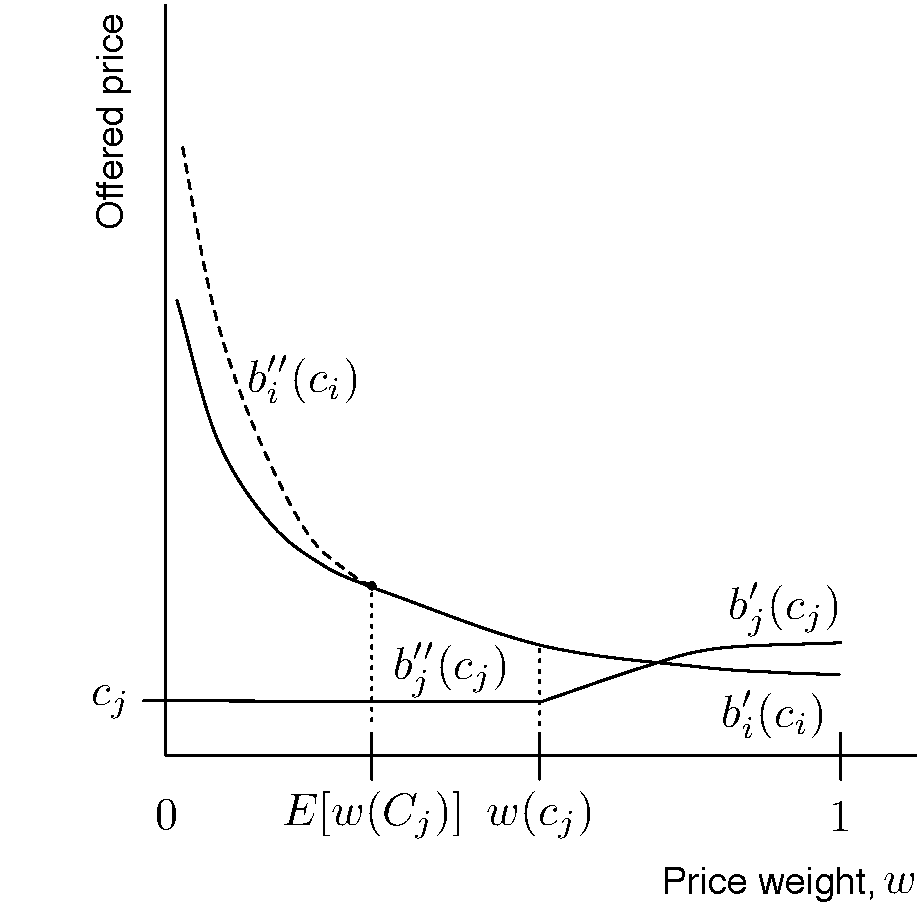
\includegraphics[width=3.5in]{Direct/Figures/pincomplete_bids_update_i_1}
	\caption{Update in bidding strategy for network operator $i$ when $w(c_j) > E[w(C_j)]$}
	\label{fig:pincomplete_bids_update_i_1_direct}
	\vspace{10mm}
	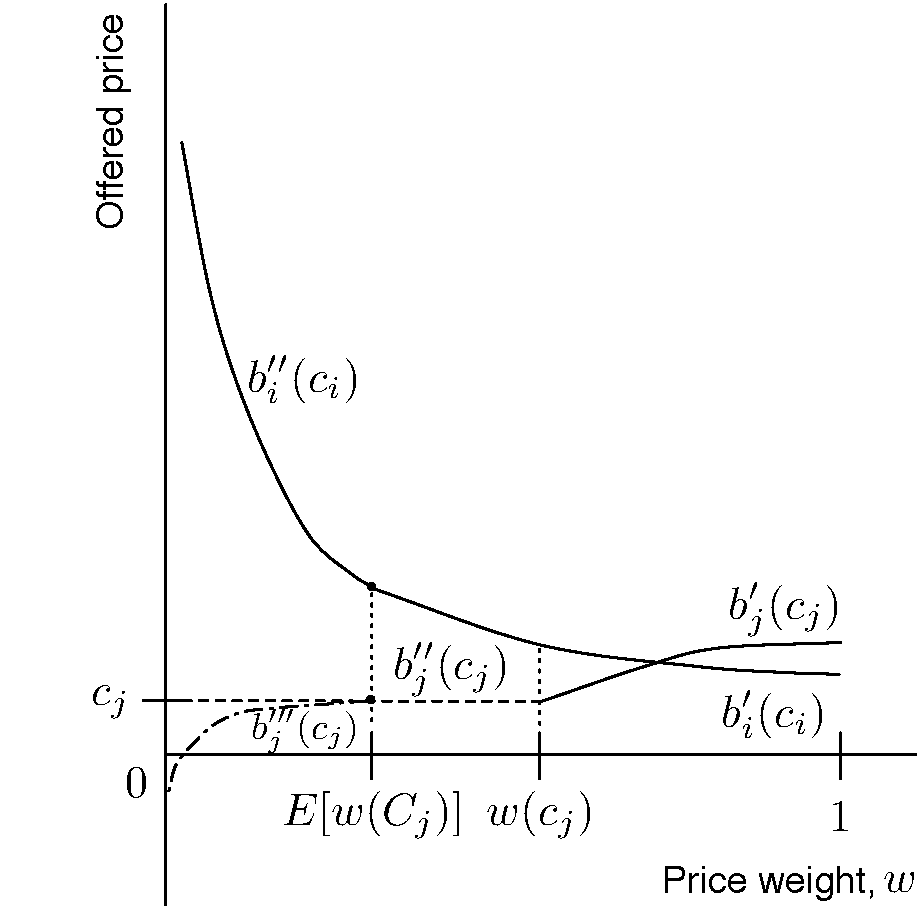
\includegraphics[width=3.5in]{Direct/Figures/pincomplete_bids_update_j_1}
	\caption{Update in bidding strategy for network operator $j$ when $w(c_j) > E[w(C_j)]$}
	\label{fig:pincomplete_bids_update_j_1_direct}
\end{figure}

\begin{figure}[tp!]
	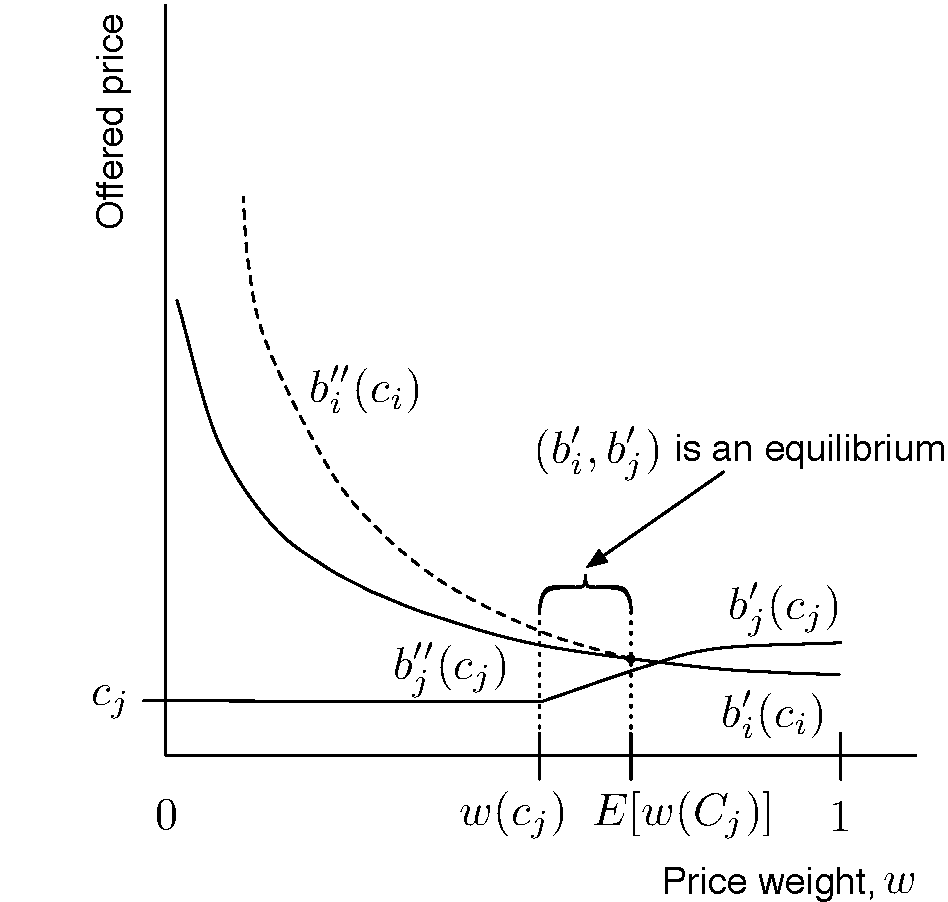
\includegraphics[width=3.5in]{Direct/Figures/pincomplete_bids_update_i_2}
	\caption{Update in bidding strategy for network operator $i$ when $w(c_j) < E[w(C_j)]$}
	\label{fig:pincomplete_bids_update_i_2_direct}
\end{figure}

Nevertheless, network operator $i$ might find it beneficial to update their bidding strategy given the fact that network operator $j$ bids according to $b_j''$ for $w<w(c_j)$, as this could potentially lead to higher profits for network operator $i$. However, there is at least one major limitation that network operator $i$ will face; that is, $w(c_j)$ as perceived by network operator $i$ is a function of cost of network operator $j$. Hence, it is a function of a random variable $C_j$. Since $C_j$ is a continuous random variable, the exact estimation of $w(C_j)$ is impossible; i.e., the probability of the event $w(C_j)=E[w(C_j)]$ is zero. Therefore, if network operator $i$ decides to update their bidding strategy, they may actually decrease their expected profits. To see why, suppose that network operator $i$ updates their bidding strategy. In this case, $b_j''(c_j) = c_j$ and $\lambda_i = 0$ which imply that $m_j = 0$, $n_j=1$ and thus
\begin{align*}
	&1 - b_i - \frac{1-w}{w}(r_i-r_j) - b_i + c_i = 0\\
	\iff &b_i''(c_i) = \frac{1}{2} - \frac{1-w}{2w}(r_i-r_j) + \frac{1}{2}c_i.
\end{align*}
If $w(c_j) > E[w(C_j)]$, then network operator $i$ will benefit from an update of their strategy; that is,
\begin{align*}
	&E\left[b_i''(c_i)-c_i \:\middle\vert\: wb_i''(c_i) + (1-w)r_i < wC_j + (1-w)r_j \right]\\
	- &E\left[b_i'(c_i)-c_i \:\middle\vert\: wb_i'(c_i) + (1-w)r_i < wC_j + (1-w)r_j \right] > 0
\end{align*}
for all $c_i\in[0,1]$ and $w < E[w(C_j)]$. Figure~\ref{fig:pincomplete_bids_update_i_1_direct} depicts the above situation. Network operator $i$ will increase their bid (or offered price) for $w < E[w(C_j)]$, and yet will not decrease their probability of winning. At the same time, network operator $j$ will not have an incentive to modify their bidding strategy as it does not yield higher profits than by bidding $b_j''(c_j)$; that is, network operator $j$ faces an optimization problem
\begin{equation*}
	\max_{b_j} E\left[b_j - c_j \:\middle\vert\: wb_j + (1-w)r_j < wb_i''(C_i) + (1-w)r_i \right],
\end{equation*}
which yields
\begin{equation*}
	b_j'''(c_j) = \frac{1}{2}c_j - \frac{1-w}{4w}(r_j-r_i).
\end{equation*}
The difference in expected profits resulting from using $b_j'''$ for $w < E[w(C_j)]$ rather than $b_j''$ is negative; i.e.,
\begin{align*}
	&E\left[b_j'''(c_j)-c_j \:\middle\vert\: wb_j'''(c_j) + (1-w)r_j < wb_i''(C_i) + (1-w)r_i \right]\\
	- &E\left[b_j''(c_j)-c_j \:\middle\vert\: wb_j''(c_j) + (1-w)r_j < wb_i''(C_i) + (1-w)r_i \right] \le 0
\end{align*}
for all $c_j\in[0,1]$. Figure~\ref{fig:pincomplete_bids_update_j_1_direct} depicts the above situation. Network operator $j$ would decrease their bid (or offered price) for $w < E[w(C_j)]$, and would bid below their cost.

If $w(c_j) < E[w(C_j)]$, then network operator $i$ will decrease their expected profits for $w(c_j) < w < E[w(C_j)]$, as in this range, the pair of bidding strategies $(b_i',b_j')$ constitutes an equilibrium. Figure~\ref{fig:pincomplete_bids_update_i_2_direct} shows the above situation. However, it is not clear whether the increase in expected profits when $w(c_j) > E[w(C_j)]$ for network operator $i$ is larger than the decrease in expected profits when $w(c_j) < E[w(C_j)]$, and hence, whether it is worth for network operator $i$ to guess the value of $w(c_j)$.

The above discussion suggests that a possible solution to the constrained optimization problem in Equation~\eqref{eq:pcomp_exp_utility_c_direct} may assume the following form
\begin{equation*}
	b_i^*(c_i) = \max\left\{ c_i, b_i'(c_i) \right\}.
\end{equation*}
However, since a formal proof is not provided, the result is stated as a conjecture.
\begin{conjecture}
\label{conj:pcomp_max_equi_bidding_str_direct}
Let there be $n=2$ network operators. Suppose $c_i$ is independently drawn from uniform distribution over the interval $[0,1]$ for all $i\in N$, and $r_i\in [0,1]$ for all $i\in N$ is common knowledge. If the optimization problem is subject to a constraint $b_i\ge c_i$, then the equilibrium bidding strategy for all $w\in (0,1]$ is given by
\begin{equation}
\label{eq:pcomp_equi_bidding_str_max_direct}
	b_i^*(c_i) = \max\left\{ c_i, b_i'(c_i) \right\}.
\end{equation}
\end{conjecture}
% subsubsection incomplete_information_n_2 (end)
% subsection direct_restricted_case_n_2_ (end)

\section{Summary} % (fold)
\label{sec:summary_direct}
In this chapter, we formally defined a game-theoretical model for the DMP auction. It was further shown that for the price weight of $w=1$, and equal reputation ratings for all bidders, $r_i=r_j$ for all $i\neq j$, the DMP auction reduces to the standard, symmetric FPA (Proposition~\ref{prop:special_case_w_1_direct} and Corollary~\ref{cor:special_case_r_i_r_j_direct}). Thus, standard results from the auction literature apply.

For the price weight of $w=0$, however, it was shown that the network operators would engage in abnormally high bidding (Proposition~\ref{prop:special_case_w_0_direct}). Hence, charging the buyer the maximum they are prepared to pay for the service.

We proposed an analytical solution to the restricted case of two network operators, $n=2$ (Proposition~\ref{prop:pcomp_equi_bidding_str_direct}). The solution is suboptimal in the sense that the derived equilibrium bidding strategies permit the network operators to bid negatively. However, it was also shown that negative bidding does not lead to negative profit for either network operator (Proposition~\ref{prop:pcomp_negative_bids_direct}). At the same time, it was proved that the network operators would not find it beneficial not to participate in the auction if they were to bid according to the strategies summarised in Proposition~\ref{prop:pcomp_equi_bidding_str_direct} (Proposition~\ref{prop:pcomp_direct_mechanism_direct}).

Finally, a constraint optimisation problem was proposed that addresses negative bidding of the bidders. However, due to technical difficulties, an analytical solution was not formally derived; but, its form was conjectured (Conjecture~\ref{conj:pcomp_max_equi_bidding_str_direct}).
% section summary_direct (end)

\section{Proofs} % (fold)
\label{sec:proofs_direct}
\begin{proof}[Proof of Proposition~\ref{prop:special_case_w_0_direct}]
Let $m = |N_0|$ be the number of network operators with the lowest reputation rating such that $m\in\mathbb{Z}_+$. Since $n = |N|$ is finite and $N_0\subseteq N$, then $m \le n$. Now, each $j\in N_0$ is facing a maximization problem
\begin{equation*}
	\max_{b_j} \frac{1}{m} \left(b_j - c_j \right), \quad\text{for all } j\in N_0.
\end{equation*}
Since $1\le m\le n$, and since $b_j\in\mathbb{R}_+$ and $\mathbb{R}_+$ is not bounded from above, this implies that the maximization problem is unbounded; that is, $b_j\rightarrow\infty$ for all $j\in N_0$.

The remaining network operators $k\in N\setminus N_0$ will try to solve
\begin{equation*}
	\max_{b_k} 0, \quad\text{for all } k\in N\setminus N_0,
\end{equation*}
since $r_k > r_j = \min_{i\in N} r_i$. Hence, each network operator $k\in N\setminus N_0$ is indifferent to the value of their bid, which concludes the proof.
\end{proof}

\begin{proof}[Proof of Proposition~\ref{prop:special_case_w_1_direct}]
The proof is analogous to the proof of Proposition~2.2 in Krishna~\cite{Krishna10}.
\end{proof}

\begin{proof}[Proof of Proposition~\ref{prop:pcomp_equi_bidding_str_direct}]
Suppose there are two network operators: network operator 1 and 2 with cost-reputation pairs $(c_1,r_1)$ and $(c_2,r_2)$ respectively. Suppose that network operator 2 follows $b_2'$ equilibrium bidding strategy. We will argue that it is optimal for network operator 1 to follow $b_1'$ equilibrium bidding strategy. First, note that $b_1'$ is strictly increasing and continuous function of cost (similarly is $b_2'$). Suppose that network operator 1 bids an amount $b_1$. Since $b_1'$ is strictly increasing, it is bijective. Therefore, there exists unique cost $c'_1$ such that $c'_1 = {b_1'}^{-1}(b_1)$. Network operator 1's expected utility from bidding $b_1'(c'_1)$ is
\begin{align*}
	&\tilde{u}_1(b_1'(c'_1), c_1) \\
	&= E \left[ b_1'(c'_1) - c_1 \:\middle\vert\: wb_1'(c'_1) + (1-w)r_1 < wb_2'(c_2) + (1-w)r_2 \right] \\
	&= \frac{1}{2} \left( 1 - \frac{2}{3}\cdot\frac{1-w}{w}(r_1-r_2) + c'_1 - 2c_1 \right) \left( 1 - c'_1 - \frac{2}{3}\cdot\frac{1-w}{w}(r_1-r_2) \right).
\end{align*}
We thus obtain that
\begin{equation*}
	\tilde{u}_1(b_1'(c_1), c_1) - \tilde{u}_1(b_1'(c'_1), c_1) = \frac{1}{2}(c_1-c'_1)^2 \ge 0
\end{equation*}
regardless of whether $c'_1\ge c_1$ or $c'_1 \le c_1$. We have thus argued that if network operator 2 follows $b_2'$, network operator 1 with a cost $c_1$ cannot benefit by bidding anything other than $b_1'(c_1)$. Similar argument can be used to show that it is optimal for network operator 2 to follow $b_2'$ while network operator 1 is following $b_1'$. Hence, $(b_1',b_2')$ constitutes a Bayesian-Nash equilibrium profile.
\end{proof}

\begin{proof}[Proof of Proposition~\ref{prop:pcomp_negative_bids_direct}]
Let there be two network operators: network operator 1 and 2 with cost-reputation pairs $(c_1,r_1)$ and $(c_2,r_2)$ respectively. Suppose that both network operators follow the equilibrium bidding strategy, $b_i'(c_i)$. We need to show that network operator 1's bid is always at least as high as their cost whenever they win or draw with network operator 2; that is, $b_1'(c_1)\ge c_1$.

First of all, note that if $r_1\le r_2$,
\begin{equation*}
	b_1'(c_1) = \frac{1}{2}-\frac{1-w}{3w}(r_1-r_2) + \frac{1}{2}c_1 \ge \frac{1}{2}(1+c_1) \ge c_1, \quad\text{for all } c_1\in[0,1].
\end{equation*}
Thus, we need only to consider the case when $r_1>r_2$.

Suppose $r_1>r_2$. If $c_1>c_2$, and since $b_1'(c_2)$ is strictly increasing in $c_1$, network operator 1 will lose for all values of $w\in(0,1]$. If $c_1=c_2$, network operator 1 will lose for all values of $w\in(0,1)$, except at $w=1$ when there will be a draw. But at $w=1$, network operator 1's bid is at least as high as her cost; i.e.,
\begin{equation*}
	b_1'(c_1) = \frac{1}{2}(1+c_1) \ge c_1, \quad\text{for all } c_1\in[0,1].
\end{equation*}
If $c_1<c_2$, it is sufficient to show that the intersection of $b_1'(c_1)$ and $c_1$ in terms of $w$ can never occur before the intersection of $\beta(b_1'(c_1),r_1)$ and $\beta(b_2'(c_2),r_2)$. First of all, we need to check that both intersections do occur; that is,
\begin{equation*}
	b_1'(c_1) = c_1 \iff w = \frac{1}{1 + \frac{3}{2}\cdot\frac{1 - c_1}{r_1 - r_2}}.
\end{equation*}
Similarly,
\begin{equation*}
	\beta(b_1'(c_1),r_1) = \beta(b_2'(c_2),r_2) \iff w = \frac{1}{1+ \frac{3}{2}\cdot\frac{c_2-c_1}{r_1-r_2}}.
\end{equation*}
Since $r_1>r_2$ and $c_1<c_2$, we have $0<r_1-r_2\le 1$ and $0<c_2-c_1\le 1$. Therefore, this implies
\begin{equation*}
	0 < w = \frac{1}{1+ \frac{3}{2}\cdot\frac{1-c_1}{r_1-r_2}} \le 1,
\end{equation*}
and
\begin{equation*}
	0 < w = \frac{1}{1+ \frac{3}{2}\cdot\frac{c_2-c_1}{r_1-r_2}} \le 1.
\end{equation*}
Now, suppose that the intersection of $b_1'(c_1)$ and $c_1$ occurs before that of $\beta(b_1'(c_1),r_1)$ and $\beta(b_2'(c_2),r_2)$. We must thus have
\begin{equation*}
	\frac{1}{1+\frac{3}{2}\cdot\frac{c_2-c_1}{r_1-r_2}} < \frac{1}{1+\frac{3}{2}\cdot\frac{1-c_1}{r_1-r_2}} \iff \frac{1-c_2}{r_1-r_2} < 0.
\end{equation*}
But since $c_2\in[0,1]$ and $r_1>r_2$ by assumption,
\begin{equation*}
	0 < \frac{1-c_2}{r_1-r_2}
\end{equation*}
we reach a contradiction, and this concludes the proof.
\end{proof}

\begin{proof}[Proof of Proposition~\ref{prop:pcomp_direct_mechanism_direct}]
Let there be two network operators: network operator 1 and 2 with cost-reputation pairs $(c_1,r_1)$ and $(c_2,r_2)$ respectively. Suppose that both network operators participate in the direct mechanism $(\mathbf{Q},\mathbf{M})$. Firstly, we show that the mechanism is incentive compatible. Without loss of generality, suppose that network operator 2 truthfully submits their cost to the mechanism. We argue that it is optimal for network operator 1 to also submit their cost truthfully. Suppose to the contrary; that is, that network operator 1 has an incentive not to reveal their cost truthfully by submitting $c'_1$. Thus, their expected utility becomes
\begin{align*}
	&\tilde{\tilde{u}}_1(c'_1) = E\left[ b_1'(c'_1) - c_1 \:\middle\vert\: 2b_1'(c'_1) - 1 + \frac{4}{3}\cdot\frac{1-w}{w}(r_1-r_2) < C_2 \right] \\
	&= \left(\frac{1}{2} - \frac{1}{3}\cdot\frac{1-w}{w}(r_1-r_2) + \frac{1}{2}c'_1 - c_1 \right)\left(1 - c'_1 - \frac{2}{3}\cdot\frac{1-w}{w}(r_1-r_2)\right).
\end{align*}
The first-order condition yields $c'_1 = c_1$ and the second-order condition is satisfied. Hence, this shows that $(\mathbf{Q},\mathbf{M})$ is incentive compatible.

Secondly, we show that $(\mathbf{Q},\mathbf{M})$ is individually rational. Since the mechanism is incentive compatible, each network operator reveals their cost truthfully. Hence, for all $c_1$
\begin{align*}
	\tilde{\tilde{u}}_1(c_1) &= \left(\frac{1}{2} - \frac{1}{3}\cdot\frac{1-w}{w}(r_1-r_2) - \frac{1}{2}c_1 \right)\left(1 - c_1 - \frac{2}{3}\cdot\frac{1-w}{w}(r_1-r_2)\right)\\
	&= \frac{1}{2}\left( 1 - c_1 - \frac{2}{3}\cdot\frac{1-w}{w}(r_1-r_2) \right)^2 \ge 0.
\end{align*}
Therefore, $(\mathbf{Q},\mathbf{M})$ is individually rational.
\end{proof}
% section proofs (end)

% chapter selling_mechanism_in_the_digital_marketplace (end)
